%% ----------------------------------------------------------------
%% Thesis.tex -- MAIN FILE (the one that you compile with LaTeX)
%% ----------------------------------------------------------------

% Set up the document
\documentclass[a4paper, 11pt, oneside]{Thesis}  % Use the "Thesis" style, based on the ECS Thesis style by Steve Gunn
\graphicspath{{Figures/}}  % Location of the graphics files (set up for graphics to be in PDF format)

% Include any extra LaTeX packages required
\usepackage[square, numbers, comma, sort&compress]{natbib}  % Use the "Natbib" style for the references in the Bibliography
\usepackage{verbatim}  % Needed for the "comment" environment to make LaTeX comments
\usepackage{vector}  % Allows "\bvec{}" and "\buvec{}" for "blackboard" style bold vectors in maths
\hypersetup{urlcolor=blue, colorlinks=true}  % Colours hyperlinks in blue, but this can be distracting if there are many links.
\usepackage{graphicx}

\newcommand{\GCxGC}{GC$\times$GC}
\newcommand{\SFCxSFC}{SFC$\times$SFC}
\newcommand{\SFCxGC}{SFC$\times$GC}

%% ----------------------------------------------------------------
\frontmatter	  % Begin Roman style (i, ii, iii, iv...) page numbering
\begin{document}

% Set up the Title Page
\title  {SFC$\times$GC}
\authors  {\texorpdfstring
            {\href{http://www.scidat.co.za}{D Malan}}
            {D Malan}
            }
\addresses  {\groupname\\\deptname\\\univname}  % Do not change this here, instead these must be set in the "Thesis.cls" file, please look through it instead
\date       {\today}
\subject    {}
\keywords   {}

\maketitle
%% ----------------------------------------------------------------

\setstretch{1.3}  % It is better to have smaller font and larger line spacing than the other way round

% Define the page headers using the FancyHdr package and set up for one-sided printing
\fancyhead{}  % Clears all page headers and footers
\rhead{\thepage}  % Sets the right side header to show the page number
\lhead{}  % Clears the left side page header

\pagestyle{fancy}  % Finally, use the "fancy" page style to implement the FancyHdr headers

%% ----------------------------------------------------------------
% Declaration Page required for the Thesis, your institution may give you a different text to place here
\Declaration{

\addtocontents{toc}{\vspace{1em}}  % Add a gap in the Contents, for aesthetics

I, Daniel Malan, declare that this thesis titled, `SFC$\times$GC' and the work presented in it are my own. I confirm that:

\begin{itemize}
\item[\tiny{$\blacksquare$}] This work was done wholly or mainly while in candidature for a research degree at this University.

\item[\tiny{$\blacksquare$}] Where any part of this thesis has previously been submitted for a degree or any other qualification at this University or any other institution, this has been clearly stated.

\item[\tiny{$\blacksquare$}] Where I have consulted the published work of others, this is always clearly attributed.

\item[\tiny{$\blacksquare$}] Where I have quoted from the work of others, the source is always given. With the exception of such quotations, this thesis is entirely my own work.

\item[\tiny{$\blacksquare$}] I have acknowledged all main sources of help.

\item[\tiny{$\blacksquare$}] Where the thesis is based on work done by myself jointly with others, I have made clear exactly what was done by others and what I have contributed myself.
\\
\end{itemize}


Signed:\\
\rule[1em]{25em}{0.5pt}  % This prints a line for the signature

Date:\\
\rule[1em]{25em}{0.5pt}  % This prints a line to write the date
}
\clearpage  % Declaration ended, now start a new page

%% ----------------------------------------------------------------
% The "Funny Quote Page"
\pagestyle{empty}  % No headers or footers for the following pages

\null\vfill
% Now comes the "Funny Quote", written in italics
\textit{``Learning is a peculiar compound of memory, imagination, scientific habit, accurate observation, all concentrated, through a prolonged period, on the analysis of the remains of literature. The result of this sustained mental endeavour is not a book, but a man''}

\begin{flushright}
Mark Pattison
\end{flushright}

\vfill\vfill\vfill\vfill\vfill\vfill\null
\clearpage  % Funny Quote page ended, start a new page
%% ----------------------------------------------------------------

% The Abstract Page
\addtotoc{Abstract}  % Add the "Abstract" page entry to the Contents
\abstract{
\addtocontents{toc}{\vspace{1em}}  % Add a gap in the Contents, for aesthetics

The Thesis Abstract is written here (and usually kept to just this page). The page is kept centered vertically so can expand into the blank space above the title too\ldots

}

\clearpage  % Abstract ended, start a new page
%% ----------------------------------------------------------------

\setstretch{1.3}  % Reset the line-spacing to 1.3 for body text (if it has changed)

% The Acknowledgements page, for thanking everyone
\acknowledgements{
\addtocontents{toc}{\vspace{1em}}  % Add a gap in the Contents, for aesthetics

I gratefully acknowledge my supervisor, Prof Egmont Rohwer, who had the faith in me to invite me to take on the project, and the patience to wait for me to respond and the patience to wait for me to finish. I am extremely grateful for the funding he supplied at the beginning of the project, when funding was a real problem. 

My thanks to David Masemula, who maintained the supply of gas cylinders.

Yvette Naud� has been a most kind and helpful lab manager.

Kobie Smit lent a kind ear to the laments, and helped me feel less alone.

Marc Bouwer, whose youthful energy proved to be highly contagious, spent hours in front of the whiteboard with me, helping to clarify thoughts and understanding basic science.

My father, Danie Malan, spent a lot of energy and time on being an instrument maker for me.

My mother, Retha Malan, made sure that feeding myself during this time was as simple as possbile.

For Sunil Patel, who, in true hacker spirit, made the \LaTeX template this document is based on freely available.

Sasol Fuel, who saw the need for expertise, and started acting as a major funding source. This freed up so many resources.

For Beyers at Chemetrix, who spent effort in keeping our outdated HP instrumentation running.

For Agilent, who supplied us with an excellent used intrument at a nominal cost.

For Barbara Lotze, for whose support I will be eternally grateful. 

Johan Erasmus, whose professional psychological help was crucial in getting me unstuck.

Dok Fanie (Dr SJ van der Walt) who was appointed as my co-supervisor, but was also my predecessor, was willing to lend an ear and encourage, supply new ideas.  "Works well when under constant supervision and cornered like a rat in a trap."

Antoinette ??insert surname of the Centre for Microscopy and Microanalysis at the University of Pretoria provided invaluable aid in performing the SEM images.

The financial assistance of the South African National Energy Research Institute towards this research is hereby acknowledged. Opinions expressed and conclusions arrived at, are those of the author and are not necessarily to be attributed to SANERI.


}
\clearpage  % End of the Acknowledgements
%% ----------------------------------------------------------------

\pagestyle{fancy}  %The page style headers have been "empty" all this time, now use the "fancy" headers as defined before to bring them back


%% ----------------------------------------------------------------
\lhead{\emph{Contents}}  % Set the left side page header to "Contents"
\tableofcontents  % Write out the Table of Contents

%% ----------------------------------------------------------------
\lhead{\emph{List of Figures}}  % Set the left side page header to "List if Figures"
\listoffigures  % Write out the List of Figures

%% ----------------------------------------------------------------
\lhead{\emph{List of Tables}}  % Set the left side page header to "List of Tables"
\listoftables  % Write out the List of Tables

%% ----------------------------------------------------------------
\setstretch{1.5}  % Set the line spacing to 1.5, this makes the following tables easier to read
\clearpage  % Start a new page
\lhead{\emph{Abbreviations}}  % Set the left side page header to "Abbreviations"
\listofsymbols{ll}  % Include a list of Abbreviations (a table of two columns)
{
% \textbf{Acronym} & \textbf{W}hat (it) \textbf{S}tands \textbf{F}or \\
\textbf{LAH} & \textbf{L}ist \textbf{A}bbreviations \textbf{H}ere \\
\textbf{FAME} & \textbf{F}atty \textbf{A}cid \textbf{M}ethyl \textbf{E}ster \\
\textbf{GC} & \textbf{G}as \textbf{C}hromatography \\
\textbf{SFC} & \textbf{S}upercitical \textbf{F}luid \textbf{C}hromatography  \\
\textbf{PWM} & \textbf{P}ulse \textbf{W}idth \textbf{M}odulation\\
\textbf{SEM} & \textbf{S}canning \textbf{E}electron \textbf{M}microscope \\
\textbf{FAME} & \textbf{F}atty \textbf{A}cid \textbf{M}ethyl \textbf{Ester} \\
\textbf{FAME} & \textbf{F}atty \textbf{A}cid \textbf{M}ethyl \textbf{Ester} \\
\textbf{FAME} & \textbf{F}atty \textbf{A}cid \textbf{M}ethyl \textbf{Ester} \\

}

%% ----------------------------------------------------------------
\clearpage  % Start a new page
\lhead{\emph{Physical Constants}}  % Set the left side page header to "Physical Constants"
\listofconstants{lrcl}  % Include a list of Physical Constants (a four column table)
{
% Constant Name & Symbol & = & Constant Value (with units) \\
Speed of Light & $c$ & $=$ & $2.997\ 924\ 58\times10^{8}\ \mbox{ms}^{-\mbox{s}}$ (exact)\\

}

%% ----------------------------------------------------------------
\clearpage  %Start a new page
\lhead{\emph{Symbols}}  % Set the left side page header to "Symbols"
\listofnomenclature{lll}  % Include a list of Symbols (a three column table)
{
% symbol & name & unit \\
$a$ & distance & m \\
$P$ & power & W (Js$^{-1}$) \\
& & \\ % Gap to separate the Roman symbols from the Greek
$\omega$ & angular frequency & rads$^{-1}$ \\
}
%% ----------------------------------------------------------------
% End of the preamble, contents and lists of things
% Begin the Dedication page

\setstretch{1.3}  % Return the line spacing back to 1.3

\pagestyle{empty}  % Page style needs to be empty for this page
\dedicatory{For/Dedicated to/To my\ldots}

\addtocontents{toc}{\vspace{2em}}  % Add a gap in the Contents, for aesthetics


%% ----------------------------------------------------------------
\mainmatter	  % Begin normal, numeric (1,2,3...) page numbering
\pagestyle{fancy}  % Return the page headers back to the "fancy" style

% Include the chapters of the thesis, as separate files
% Just uncomment the lines as you write the chapters

% Chapter 1

\chapter{An introduction to biodiesel} % Write in your own chapter title
\label{Chapter1}
\lhead{Chapter 1. \emph{Biodiesel}} % Write in your own chapter title to set the page header


\section{Resources}

A midden is an archaeological feature of prehistoric human life, consisting of all the stuff that a household or community discarded, all on a pile. The excavation of middens can tell archaeologists a lot about diets and customs of prehistoric people.

The midden is a sign that humans have, since the dawn of civilisation, had a problem with discarding of the remnants of resources. Today we  might not have the same problem near our homes, but our landscape is littered with mine dumps and ash dumps from power stations. We use up resources and the waste of that usage alter our world.

The discovery in the 1800s of the internal combustion engine and the discovery that it can be fueled by plentiful and cheap petroleum might have seem like a break from this cycle. The oil was pumped from the ground, and after processing all of it was used in engines, and the remnants was a gas that was exhausted into the air and disappeared. 

But the sad thing was, this didn't work for very long. The carbon cycle had been elucidated by Priestly in 17xx, and it was soon realized that the carbon dioxide would build up in the atmosphere. Arrhenius was the first to make the connection between the rising carbon dioxide levels in the atmosphere and a possible increase in the atmospheric temperature.

\section{Introduction to Biodiesel}

Biodiesel is a diesel fuel, in other words it is a fuel for compression-ignition internal-combustion piston engines. It is derived from fats and oils, and is therefore biologically based. Because plants and animals obtain their fats and oils from photosynthesis biodiesel has the potential to be a carbon-neutral fuel, which is to say it is one that will not contribute greenhouses gases to the atmosphere.

While diesel engines can be run on vegetable oils directly, there are technical problems associated with it. However, the conversion of the triglycerides of the oil to a mixture of fatty acid esters is a simple reaction, well understood, and easy to implement. This reaction is known as a transesterification, since the glycerol ester of the fatty acids is turned into a methanol ester. 
\begin{figure}[htbp]
	\centering
	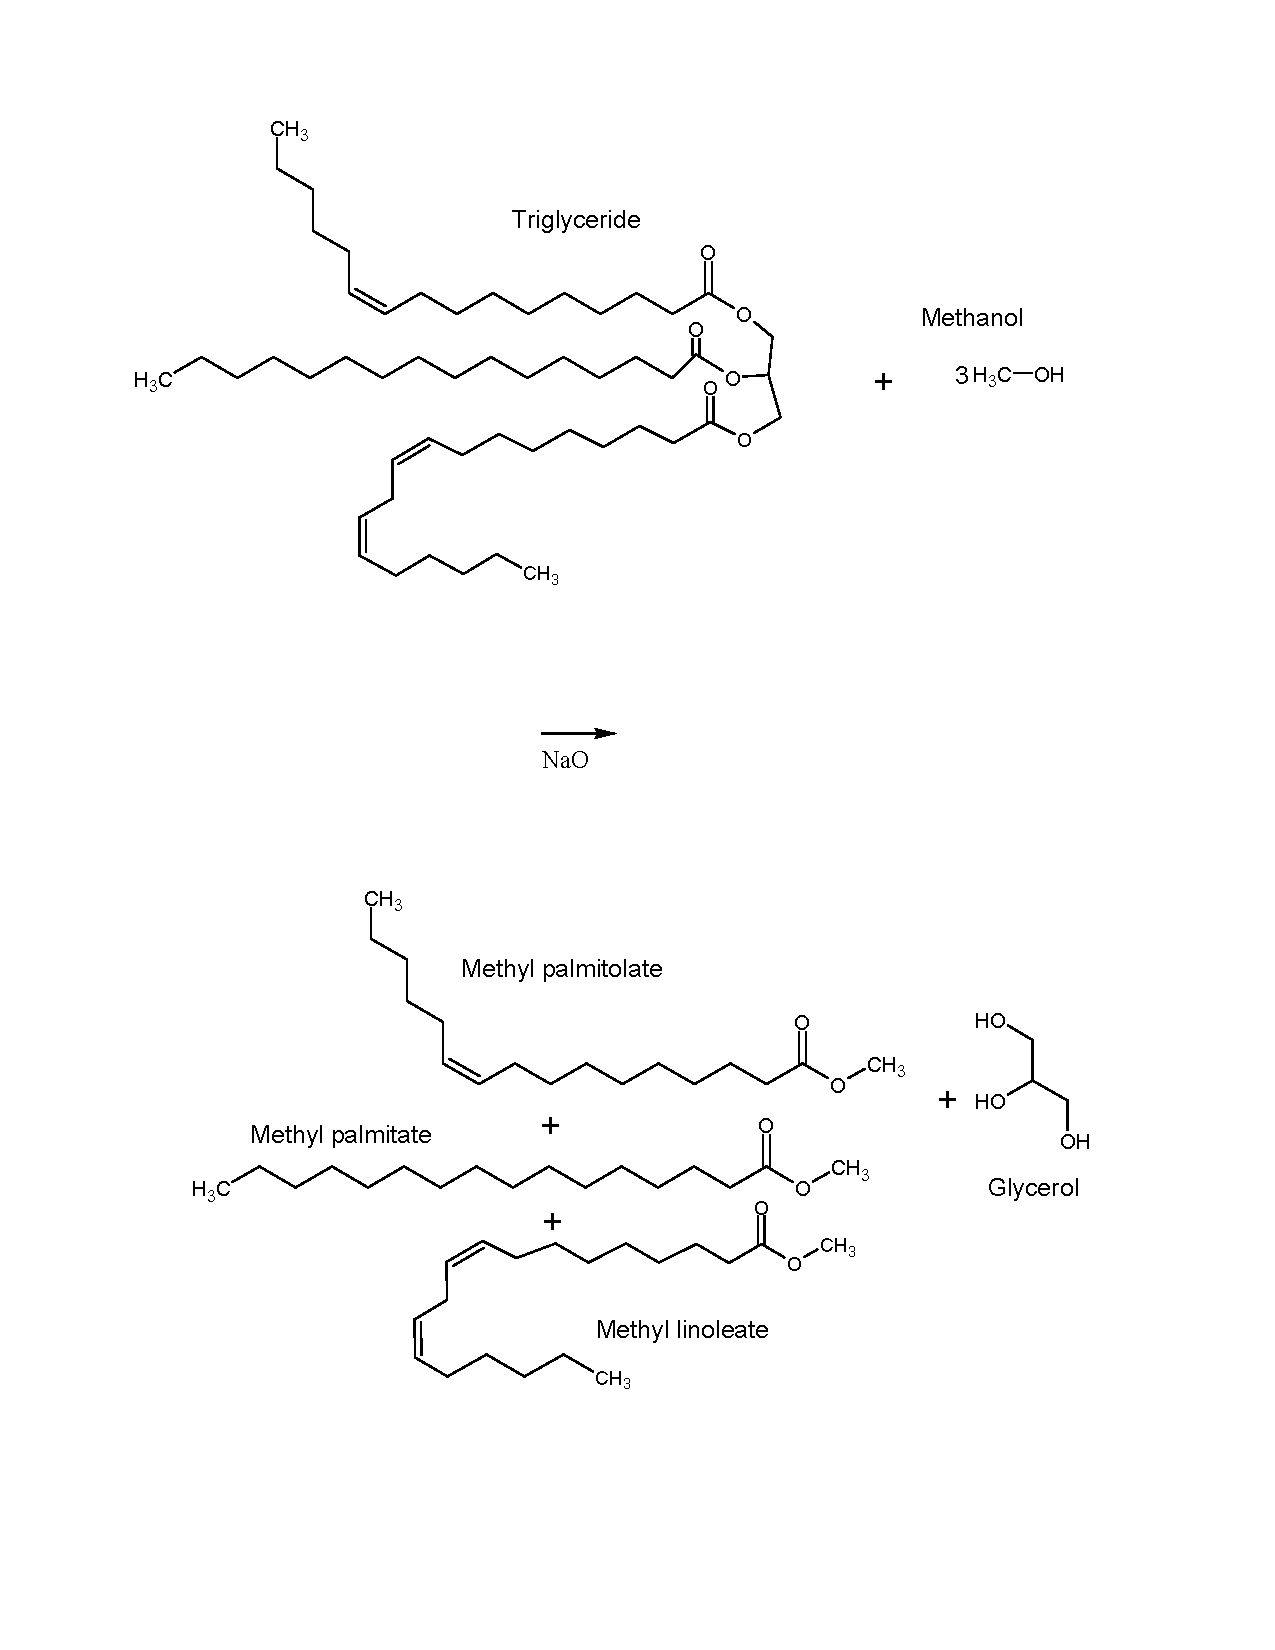
\includegraphics[width=0.8\textwidth,natwidth=4.17in,natheight=3.32in]{./Figures/Transesterification.pdf}
	\rule{35em}{0.5pt}
	\caption[Transesterification]{Transesterification of acyl triglycerides.}
	\label{fig:Transesterification}
\end{figure}

This transesterification turns the oil into a mixture of fatty acid esters that has a lower viscosity and other physical properties that makes it suitable for use as a diesel fuel. 

There are a few things to note about this picture:
\begin{itemize}
	\item Some of the fatty acids have double bonds, some not. In general, the fewer the number of double bonds, the easier it is for the straight chains to crystallize, and by implication, the higher the melting point. 
	\item The fatty acid chains can have different lengths. In common fats and oils the number of carbon atoms vary between 12 and 20. The longer the chain the higher the melting point.
	\item The different fatty acids can sit on different positions on the glycerol backbone.
	\item.Each fat molecule can have different 
	\item It is a three-step reaction, and production is thermodynamically controlled. Therefore there are intermediates in the reaction mixture, also diglycerides and monoglycerides.
	\item The polar methanol reagent and the nonpolar oil or fat are not miscible, and neither are the glycerol and the FAME products. Therefore the reaction needs mixing for the reaction to take place, but also waiting for the products to separate, and the reaction mixture is usually heated to reduce the viscosity and facilitate mixing. 
	\item The reagents and the products are miscible. Since the reagents can't be tolerated in the product, this implies that the reaction must be pushed to completion by choosing appropriate reaction conditions. 
	\item The methanol reagent is very inexpensive because it is usually obtained from the petroleum industry. This portion of the biodiesel is therefore not carbon neutral. 
	\item The glycerol is a side product with very little value, and at the moment it needs to be disposed of. 
\end{itemize}



\section{Biodiesel production}

The basic transesterification reaction of biodiesel is quite simple. The feedstock fat or oil is mixed with an excess of methanol, and a catalyst is added, and the reaction mixture is heated and stirred. Under these conditions the equilibrium of the transesterification reaction lies far over to the product side of the reaction, and the biodiesel is formed. The reaction products, glycerol and biodiesel, are also not miscible, and the two separate into layers, FAMEs at the top and the glycerol at the bottom. The glycerol is drained off and the biodiesel is washed with water to remove catalyst remnants and methanol. 

The feedstock of biodiesel can be almost any fat or oil. Vegetable oils are preferred, because they can be farmed. Animal fats can be used, and from a dietary point of view the reduction of animal fats in the national diet would improve public health, the carbon intensity of the production of animals is very high, and more carbon emission reduction can be achieved by not breeding animals than by using their fats as fuel. At best, animal fats as feedstock should be seen as a sink for waste animal products. A recent example of this is a proposal to render the daily 8 tonnes of chicken carcasses from the daily natural deaths of layer chickens in the Namakkal district in Tamil Nadu state in India, which could deliver enough rendered chicken oil produce 800000 litres of biodiesel per year. (There is already a ready market of chicken meal for feed and fertilizer.) \cite{Abraham2013} \cite{Ananth2013}

Not all feedstocks are created equal. The promotion of biodiesel is a political tool, and therefore some are considered better than others. in the USA soybean oil is the main feedstock, mainly because the National Biodiesel Board is controlled by soy interests, and owns the safety data that allows certified biodiesel to be sold on the open market\cite{Estill2005}, keeping other feedstocks out of the market. In Europe, especially Germany, rapeseed oil is the main feedstock, because it keeps German farmers on their land. The European order of things is a bit more democratic, so anybody who can produce biodiesel from any feedstock, although some are less likely to receive government support than others.

One of the few undoubtedly good feedstocks of biodiesel is used vegetable oil. Vegetable oils that are used for frying food deteriorate with use, and good practice, enforced by many governments, don't allow the oil to be used for food beyond a certain point. Ordinarily this oil would then be discarded in landfill, were it would eventually be broken down by microorganisms to carbon dioxide and water. But the used oil can be collected by the biodiesel industry and converted into fuel, which can then power vehicles. 

This sounds like a good idea, except that the soap industry also depends on waste vegetable oils and waste fats. Lacking a source of oils for the cosmetic and cleaning industry, they might turn to synthetic surfactants, wholly made from fossil carbon.

The catalyst most often used in the transesterification is sodium hydroxide or sodium methoxide. This is the cheapest available catalyst. Unfortunately the spent catalyst is also a waste product, and it contains sodium. For countries near the sea the sodium waste is not a problem since they can pump it into the sea with little concern. In South Africa, the disposal on land of sodium is forbidden, so disposal becomes a huge cost. Acids catalysts are also used, and have the added benefit that they will esterify free fatty acids, but the reaction is much slower than that of the base catalysis. In an industry where most reactions are done in batch conversions the slowness is undesirable.

There is a lot of research being done on heterogeneous catalysts for biodiesel. In general, however, the catalytic efficiency is low, and not all of the oil gets converted, and the catalysts need to be regenerated. In the style of catalyst development this is nothing new, and without doubt the quality of the catalysts will improve as time goes by, but

Another promising development in biodiesel production is the use of supercritical methanol. In supercritical methanol the methanol is at high pressure and temperature, and the properties of it change, so that it becomes a solvent for the feedstock oil. The reaction can then take place in a homogeneous mixture, which speeds up the reaction considerably, because the rate-limiting effect of mass transfer across a phase interface is eliminated. When the pressure in the reaction vessel is released, the solvent properties of the methanol change again, and the biodiesel and the methanol/glycerol solution separates. The methanol and the glycerol can be separated by a simple distillation, and there is no spent catalyst to get rid of. 

Feedstocks contain different contaminants. Free fatty acids is one common one, because in any oil there are some free fatty acids. An abundantly available feedstock, rice bran oil, is not used for biodiesel because of the high level of free fatty acids. Although there are technological fixes for this, the increased complexity in the production process increases the price of the biodiesel, making it uncompetitive with petrodiesel.

Most feedstocks also contains other, non-oil lipids. The tocopherols is one, a common natural antioxidant found in cell membranes. This might provide an antioxidant effect to the biodiesel too. The phospholipds that make up cell membranes are also present, and because they have a detergent effect are sometimes a major problem. Biodiesels often retain the colour of their parent feedstock, because the pigments that provide the colour are perfectly oil-soluble, and are equally at home in the feedstock oil and the finished biodiesel.

\section{The chemical analysis of biodiesel and SANS 1935}

While the fuel industry had some time to get used to the requirements posed by a good diesel fuel, and some of those can be carried over to biodiesel, biodiesel and petrodiesel are very different chemical mixtures, and consequently have different requirements.

In response to this, there had been starts made to setting up standards of good biodiesels. The Americans have the ASTM D6751, and the Europeans wrote EN 14214. Interestingly, the US standard only cover biodiesel as a blend feedstock, while the European standard applies to biodiesel as both an ``extender'' and a pure fuel. 

In South Africa SANS 1935 \cite{SANS1935} was adopted. This is essentially a copy of the European standard, with minor adjustments made to accommodate the most likely South African feedstock of large-scale biodiesel production, soybeans.

Below follows a point-by-point explication of the meaning and implications of the content of SANS 1935

\subsection{1 Scope}

This paragraph explains the scope of the standard, \textit{i.e.} that it applies to biodiesel, which is a diesel fuel or a diesel fuel blend component.

\subsection{2 Normative references}

This section contains a long list of standards referred to in this method. 

\subsection{3 Definitions}

This short section defines two terms: \textbf{additive} and \textbf{ biodiesel}.

\subsection{4.1.1 The automotive biodiesel fuel shall contain, principally, mono-alkyl methyl esters of long chain
fatty acids derived from vegetable oil.}

This clause pins biodiesel down as quite a particular product. While this makes it easier to write the standard, it also might stifle innovation. Specifying methyl esters, for instance, precludes the use of ethanol as alcohol in the transesterification. It's a fact not often mentioned in the discussion of biodiesel as a green product that the methyl group in the biodiesel molecule is practically universally derived from the petroleum industry. Its low price and abundant availability make a hard economic argument against the adoption of another alcohol, but while this is the case biodiesel cannot be described as a sustainable fuel. 

The phrase mono-alkyl methyl ester is not a good phrase to use, and I believe it to be the result of an editorial mishap. 

\subsection{4.1.2 Suitable fuel additives without known side effects may be used to help avoid deterioration of
driveability and emissions control durability. Other technical means that exhibit an effect equivalent to
that of additives can also be used.}`

This clause enables manufacturers to invent modifiers to give the fuel more desirable properties.

\subsection{4.1.3 The fuel may contain small quantities of colouring materials which are documented as harmless
to give it a distinctive colour.}

This clause allows manufacturers to differentiate products, help prevent mistakes, and is sometimes used to identify fuel, \textit{e.g.} fuel with a different taxation rate.

\subsection{4.1.4 The fuel shall be clear and free of visible water, sediment, suspended matter and any other
contaminant that is documented as likely to cause malfunctioning of equipment designed to use this
type of fuel, either as a blend or in its 100 \% concentration form.}

This is just stating the obvious, in effect declaring that a fuel sold as biodiesel is fit for use, and also provides blanket protection against contaminants not otherwise specified.

\subsection{4.2 Physical and chemical properties
The fuel shall comply with all the requirements given in table 1.
NOTE 1 In case of a need for identification of biodiesel, it is recommended that a method based on the
characterization of fatty acid methyl esters by LG/GC, in accordance with EN 14331, be used.
NOTE 2 In case of a need to identify the source oil of biodiesel, the iodine value of the biodiesel can be calculated
by the method presented in annex B.}

This sort paragraph is actually the meat of the standard. It refers to Table 1 of the standard, which is discussed in detail on page \pageref{table1} below.

\subsection{5.1 For all tests, use samples taken in accordance with annex D.}

This draws attention to the fact that doing chemical tests for commercial purposes need to ensure that the sample is actually representative of the bulk. It would be easy to take a single sample from a bulk container in such a way that it would be sure to pass or fail the test. For example, a bulk fuel tanker could contain a minuscule amount of water at the bottom of the tank. If a simple sample were to be taken by means of a draining cock, this small sample would contain a relatively large amount of water, violating the standard, while the bulk of the sample might actually be of very good quality. A representative sample would provide a meaningful average of the whole. 

\subsection{5.2 For all properties, use the applicable test method or, when relevant, one of the applicable test
methods listed in column 3 of table 1}

This points to the fact that standardized methods should be used, and that not all tests are equal in accuracy and precision.

It also protects the testing laboratory, because if a new problem should be developed with the fuel's quality assessment, and the problem had not become apparent in well-performed analytical tests specified by the standard, the laboratory would have performed all the legal steps to ensure quality. Ethical considerations would have to be considered on a case by case basis, because a problem with a fuel might have been apparent to test laboratory staff that did not show up in the tests.
	
\subsection{5.3 The limiting value for the carbon residue given in table 1 is based on product prior to the addition of ignition improver, if used. If a value exceeding the limit is obtained on finished fuel in the market, use ISO 13759 to determine the presence of a nitrate-containing compound. If an ignition improver is thus proved present, the limit value for the carbon residue of the product under test cannot be applied. The use of additives does not exempt the manufacturer from meeting the requirement of maximum 0.30 \% mass fraction of carbon residue prior to the addition of additives.}

This is a methodical sidestep of a known chemical interference that cannot be controlled for using existing methods.

\subsection{5.4 Precision and dispute}

This section talks about precision, and how dispute should be resolved. Discussion of it falls beyond the scope of this chapter.

\subsection{6 Packing, marking and placarding}

This section deals with the packing of biodiesel in containers. Basically it should be packed in drums and tanks that does not leak, the tanks and drums should be labelled properly, and that road freight standards apply if biodiesel is transported by road. (I wonder why transport by rail is not mentioned. Is this oversight, ignorance, or does the railway apply its own standards? In any case it seems a bit like the highly efficient (in terms of carbon emissions) train transport system is being ignored again)

\subsection{Annex A: Precision data}

Any test method yields a result, with the result being true only to a certain degree. This degree of trueness is given by the precisions. This table is included because the precisions given for the established standard values might differ slightly if it is applied to other materials.

\subsection{Annex B: Calculation of iodine value}

Iodine value is a very old technique for determining the degree of unsaturation of fats and oils. I have the feeling that somebody on the committee, some crotchety oldster, insisted on including iodine value in the table of specified values. The younger and more advanced members of the committee added this annex to get something more advanced in. ``In the case of dispute on the iodine value this method shall be used as a substitute for EN 14111''. This sentence seems to indicate that chromatographic technique specified here is superior to the iodine value method. 

Of course the iodine value of EN 14111 is simpler to implement than the chromatographic method of EN 14103, but since EN 14103 will be performed in any case, the redundancy doesn't seem to make sense. Knothe \cite{} seem to think so too.

\subsection{Annex C:(normative) Correction factor for calculation of density of biodiesel}

This correction is an aid to the testing lab. It is much easier to measure a density at an unspecified (but fixed) temperature than it is to do it at a specified temperature. This correction makes it easier to apply the test.

\subsection{Annex D: (normative) Sampling and compliance with this standard}

This annex provides the technical details of the section 5.1 of the standard.

\subsection{Annex E: Quality verification of automotive biodiesel fuel}

This Annex is an advertisement for the ISO 9000 quality assurance system.

\subsection{Table 1}

Here follows a detailed discussion of the contents, relevance and methods of Table 1 of SANS 1935.
\label{table1}
\subsubsection{Ester content}

This is the ester content specified: 96.5\% This does not leave much space for other stuff, but leaves some room for contamination of fuel-valued components. It is interesting that this line does not specify that the esters should be methyl esters, but that is covered in section 2.1 of the standard. The footnote specifies that the other 3.5\% may only be additives, and not any non-FAME material.

\subsubsection{Density}

The fuel's density is specified, as the mass per unit volume. This is necessary, because fuel quantities can be specified in either volume or mass, and there needs to be a good relationship between the two. 

The density of the fuel also determines its energy density.

\subsubsection{Kinematic Viscosity}

This is a very important specification. 

The kinematic viscosity of a liquid is its viscosity divided by its density. This gives a number that can be used in calculating its flow properties under dynamic conditions.

If the viscosity is too high, the injectors in the engine might not be able to inject the right amount of fuel, because of the metering of the pump is based on timing, and if the flow is not as expected the metering will not be as expected.

If the viscosity is too high, the droplet-forming mechanism is not as effective. In this process, surface tension of the liquid fuel pulls the droplets into spherical shape. The faster the surface tension can act, the smaller the droplets can be. The rate of flow of the liquid is limited by its viscosity, which makes a defined viscosity necessary for the proper operation of the engine.

If the viscosity is too low, there might be other problems. The injection process in the diesel engine uses very high pressures to produce a fine enough spray of fuel into the combustion chamber. While a lower viscosity is preferable for producing a better spray, once again the volume delivered is measured by time, and if the flow is higher than expected, the amount of fuel will be too much. There is also the problem of reverse flow. In the injector the piston of the pump is not sealed, because it is not usually necessary, so it is not a positive displacement pump. If the viscosity of the fuel is too low, more fuel than expected will flow past the injector piston back into the system, and less will be injected into the engine. This problem would not apply to common-rain engines.

Nevertheless, the range of viscosities are large enough to accommodate a wide variety of feedstocks to be used, from heavy palm oil to light sunflower oil.

\subsubsection{Flash Point}

The flash point of a flammable liquid is that temperature of the liquid where a flame applied to the vapour above the liquid is transferred to the liquid itself.

The flash point of biodiesel is naturally much higher than petrodiesel. In the manufacturing process, however, there might be highly flammable methanol left in the final biodiesel product, which would decrease its flash point dramatically. 

\subsubsection{Sulfur Content}

One of the pollutants from petrodiesel, and from coal and petroleum combustion in general, is sulfur dioxide. When this mixes with rainwater it forms sulfurous acid, and acidifies the rainwater, forming what is known as acid rain. This is toxic to plants and has the potential to damage ecosystems. Legislation and regulation have steadily decreased the permissible amounts of sulfur emissions. This is fairly easy to implement in stationary plants such as power stations, but in vehicles it prove to be more expedient to limit the amount of sulfur in the fuel, regulating the emissions that way. South Africa has only recently introduced low-sulfur diesel.

Biodiesel is naturally sulfur-free, so this limit would mostly prevent the use of sulfur-containing additives, and the occasional odd feedstock with high sulfur content.

\subsubsection{Carbon Residue}

Biodiesel is a fairly non-polar liquid, and therefore a good solvent for other compounds. Some of these compounds might be solids, so that when the fuel evaporates there may be a residue. These solids could tend to accumulate in some part of the fuel system or engine, causing improper function or damage. (Note that the carbon residue have a fuel value, and its presence does not detract from the biodiesel's value as a fuel.) This test puts a limit to these dissolved solids. 

\subsubsection{Cetane Number}

This number points to the fuel's suitability as a diesel fuel. At a low cetane number, the fuel evaporates and ignites too easily, causing detonation, called pinging or knocking. Beyond a certain cetane number, however, there is no change in performance.

The cetane number is usually determined in a test engine, and this is a fairly specialized test.

\subsubsection{Sulfated Ash Content}

Ideally a fuel will burn completely into gaseous compounds, and if it were composed entirely of carbon compounds and the combustion process was perfect it would. However, the feedstocks of biodiesel naturally contains some non-carbon compounds, and these will not necessarily vaporize during combustion. This would then remain in the engine, possibly causing deposits, altered operation and possibly damage.

In this test a sample of the fuel is digested with sulfuric acid, and the remnants heated. The remains is ash, and represents the non-combustible portion of the fuel. This paragraph specifies a limit to ash.

\subsubsection{Water Content}

Water in fuel is of great concern. In combustion it robs energy, in storage it promotes corrosion, it permits growth of bacteria, in increases solubility of ash-forming compounds.

Biodiesel is more hygroscopic than petrodiesel, and therefore the limits on water need to be set stricter.

Water in biodiesel can be determined by the Karl Fischer titration usually used in petroleum analysis.

\subsubsection{Total Contamination}

I don't know what this means. It seems to be taken over from the petrodiesel methods. The standard notes in a footnote that ``Pending development of a suitable method, EN 12662 shall be used.'' This seems to show that it is not deemed very important, but worth looking at.

I suppose the total contamination would be all the things in the fuel that are not FAMES or additives.

\subsubsection{Copper Strip Corrosion}

In this test clean copper strips are immersed in the biodiesel for three hours at 50 $^\circ$C. After this time the copper strips are visually inspected, and the amount of corrosion judged, compared to standard strips. This is a practical test of the corrosive properties of the biodiesel. If the fuel causes excessive corrosion in fuel systems it could cause leaks in storage tanks and transfer lines, and in the engine it could lead to excessive wear and engine failure.

\subsubsection{Oxidation Stability}

Biodiesel should be stable against oxidation in the air. This is a measure of its shelf life. Oxidation of the biodiesel causes the chemicals it is made of to change its composition, and therefore it might no longer conform to specification. Oxidation of the fuel increases its acid value and increases the cetane number, but otherwise it has little impact on the usability of the fuel.

The oxidation stability is another practical measure. It is done in an apparatus called the Rancimat. In this apparatus the sample of biodiesel is heated while a stream of oxygen is bubbled through. The air stream is captured from the sample and then bubbled through water in a conduction cell. The conduction in the conduction cell depends on the volatile polar compounds give off by the heated sample. Under ordinary circumstances there are no volatile compounds coming off biodiesel. With time and heat, however, the sample starts to oxidize, and some of the oxidation products are volatile and polar, and in addition, catalyses the oxidation. After an induction period therefore, oxidation starts and rapidly accelerates. This oxidation can be observed as a sudden increase in the conductivity of the water in the conductivity cell.

This method and apparatus has been transferred from the food industry, where it has been used in the determination of the resistance to oxidation of fats and oils.

It is fairly important that biodiesel have a good stability at high temperatures too. In modern common-rail engines the diesel fuel is circulated in the injection system on or near the hot engine block, and the fuel might stay at these high temperatures for an appreciable time before it is injected.

\subsubsection{Acid Value}

The acid value gives an indication of the acidity of the biodiesel. High acidity is of course associated with high corrosion.

The cause of too-high acidity can be either left-over acid catalyst, or by high levels of free fatty acids. Some biodiesel feedstocks, like rice bran oil naturally contains many free fatty acids. Free fatty acids are also a source of carbon residue, because they are non-volatile: some of them are even solids at room temperature.

\subsubsection{Iodine Value}

The iodine value of the biodiesel is a measure of the degree of unsaturation of the fatty acids of the biodiesel. As discussed above, the inclusion of this measure in the standard is of doubtful utility. Perhaps it was introduced to protect the European rape seed farmers from the possibility of the importation of cheap soy-based biodiesel from the USA, because the limit in the original European standard is much lower than in the South African standard, where it had to be increased to accommodate the likelihood of soybean-based biodiesel. 

On the other hand, the setting of this value has made palm oil (which is a highly saturated oil) a good feedstock for European biodiesel, and therefore tropical countries have started to produce palm oil specifically for the European export market. This is unfortunate, for in some countries, Malaysia being a prime example, rainforests were being replaced by oil palm plantations.

\subsubsection{Linolenic acid methyl ester}

Linolenic acid is a doubly-unsaturated fatty acid with a chain of 18 carbon atoms. Its methyl ester is a valid compound in the fuel, and therefore the limit is very high at 12\% mass fraction. However, because of the double unsaturation including an allylic carbon atom it is especially vulnerable to oxidation. Keeping the quantity of this FAME low helps promote a stable fuel with a long shelf-life.

The specification of linolenic acid in this context is unfortunate, because it is not the only unstable fatty acid with allylic double bonds. It might therefore be possible to produce an unstable fuel that conforms to the specification. 

\subsubsection{\texorpdfstring{Polyunsaturated ($geq$ 4 double bonds) methyl esters}{Polyunsaturated methyl esters}}

No more than 1\% of the FAMEs in biodiesel may have more than four double bonds. This is once again a matter of stability and shelf-life, and therefore the limit is set very low. 

It is also to prevent fish oil from being used as a feedstock for biodiesel production. This is a good thing, because the world's fisheries are in a perilous state, and to allow fuel for an excessive lifestyle to be produced from this scarce resource would be near criminal.

It is interesting to note that this limit is one for which no test has been prescribed, because none exists yet.

\subsubsection{Methanol content}

No more than 0.2\% of the biodiesel may be methanol. Methanol is one of the feedstock products in biodiesel production, but it adversely affects the performance of the fuel. It lowers the viscosity and the flash point and decreases the cetane number. It might mask viscosity problems, which would appear if the methanol evaporated during storage.

Besides, the methanol is one of the non-renewable portion of the fuel, so it should be used very sparingly.

Ordinarily there would not be much methanol left in biodiesel, because it separates from the biodiesel and up in the glycerol layer. An excess of methanol in the finished biodiesel would indicate some emulsifying effect of some contaminant, or another chemical problem with the fuel.

\subsubsection{Monoglyceride content}
\subsubsection{Diglyceride content}
\subsubsection{Triglyceride content}

These three go together. The reaction of the production of biodiesel is a three-step reaction, where the three fatty acids attached to the glycerol backbone are picked off one by one and methylated. 

Like this: 	\\Triglyceride + MeOH $\rightarrow$ Diglyceride + FAME\\
		Diglyceride + MeOH $\rightarrow$ Monoglyceride + FAME\\
		Monoglyceride + MeOH $\rightarrow$ Glycerol + FAME 
		
Because these are equilibrium reactions, there are always some of the starting compounds left in the final mixture. The mono-, di- and triglycerides are besides this also soluble in the FAMEs. This makes a great possibility for contamination by these side-products. This then also test is also a test to make sure that the reaction had run to completion.

These are also the compounds that are responsible for injector coking and other problems, so their control is important. 

Because the last is the one that is most difficult to drive into an equilibrium where the products are in excess, the limit on monoglycerides (0.8\%) is higher than the 0.2 \% limit for the tri- and diglycerides.

\subsubsection{Free glycerol}

Glycerol is the side-product of the reaction, and it is definitely not a wanted compound in biodiesel. It increases the viscosity of the fuel and makes it more hygroscopic. It provides nutrients for organisms like algae and bacteria that colonizes fuel tanks.

As can be expected from the number of hydroxyl groups that can form strong hydrogen bonds, glycerol is denser than the FAME esters, and separates out under gravity. If not enough settling time is allowed, though, or there is a problem with emulsification, the glycerol content of the biodiesel may exceed the low 0.02 \% limit.

\subsubsection{Total glycerol}

Total glycerol includes the free glycerol and the glycerol bound to the mono-, di-, and tri-glycerides. Since this limit is quite high (0.25 \%) compared to the 0.02 \% in the Free Glycerol test, it seems that bound glycerol is much more tolerable. 

Including total glycerol seems redundant, because the limit would never be reached if all the glycerides are under control.

\subsubsection{Group I metals (total of Na and K)}

Fatty acids that are neutralized by alkali bases form soaps. These are molecules that consists of a fatty acid conjugate base and an alkali metal atom. These are not particularly soluble, promotes the forming of emulsions and increases ash content. 

Of course sodium and potassium hydroxide are used in the base catalysis of the transesterification process. 

The problem with fatty acids are that they form a natural component of many feedstocks, and that soap formation is then a natural side-product of the transesterification. The free fatty acids can be esterified in a separate acid-catalysed process. This play some role in the economics of biodiesel, because it makes low-FFA feedstocks desirable.

\subsubsection{Group II metals (total of Ca and Mg)}

Calcium and magnesium hydroxides can also be used as catalysts, but are also naturally present in plants. The are also ash-forming compounds, so controlling for their presence.

Testing for these alkali and alkali earth metals are a test of sufficient washing of the biodiesel and the proper use of the correct amount of catalyst. 

\subsubsection{Phosphorous content}

I don't know exactly why the test for phosphorous, but it is a natural constituent of plants. Its oxides are acidic, so it will play a role in exhaust system corrosion if it got burned up in the engine. It will probably contribute to acid rain too, although the phosphorous compounds are not particularly volatile and therefore won't spend much time in the atmosphere.

\subsubsection{Cold Filter Plugging Point}

Petroleum products are mixtures, and therefore petrodiesel does not have sharply defined melting point. However, it does become solid at low temperatures, low being temperatures typically found in terrestrial winters. To ensure that the fuel remains liquid at all likely temperatures it us usual to specify some temperature above which the fuel should still stay liquid. 

Traditional measures include the ``cloud point'', the temperature where visible crystals first start appearing in the oil, giving it a cloudy appearance, and the ``pour point'', the temperature at which the oil can no longer be poured from a container. However, at the cloud point the fuel is still quite liquid, and usable as a fuel, so the cloud point does not give a good indication of suitability. So the compilers of EN 14214 settled for a more practical point, and uses the ``cold filter plugging point''. This is the temperature at which the biodiesel will contain enough solid material to plug a specified filter. This is used because the fuel system only need to pump the fuel through the fuel filter under cold conditions. 

In the European standard EN 14214 the temperatures and dates for which they apply are left to member countries to specify, since the standard needs to be applicable from Sicily to Finland.

SANS 1935, however has an easier task, and the cold filter plugging point (CFPP) is specified as -4 $^\circ$C in winter and +3 $^\circ$C in summer, and then goes on to say in a footnote. ``Winter shall be considered as being from 1 April to 30 September and summer shall be considered as being from 1 October to 31 March.''

\subsection{Conclusion}

The standard SANS 1935 then gives a long list of criteria to which a biodiesel must conform before it can be sold on the open market. There seems to be some redundancies and perhaps one or two contradictions in the standard, but in general the intent and its application is acceptable. It reflects the knowledge of the time it was written, and in future one will perhaps see an improved and more up-to-date version.

I will have to make a study of the numbers in the standard to see how they add up to a total biodiesel budget.

There is much that can be done to understand biodiesel chemistry better. The role of additives can be examined much further. Particular areas of concern are oxidative stability, where the use of anti-oxidants can be explored, and studies to understand the coking of injectors better

 % Introduction

% Chapter 2

\chapter{Literature Background} % Write in your own chapter title
\label{Chapter2}
\lhead{Chapter 2. \emph{Literature}} % Write in your own chapter title to set the page header

\section{Introduction}

In trying to make sense of what to write in this Literature Review, and thrashing around for a bit, I discovered Randolph's paper \cite{Randolph2009}, which contains Table~\ref{tab:TaxonomyOfLiteratureReview}. While Randolph's and Cooper's papers are written for an audience of social scientists I think it is a worthwhile paper to follow for in my experience social scientists are much more rigorous in researching their research questions than natural scientists. 

I think it will be of assistance to the reader if I explain what to expect in the review, and why.

The \emph{focus} of the rewiew will be on ``practices or applications'', since our goal is to develop practical new instrumentation. 

It's \emph{goal} will be the ``identification of central issues'', because we want to discover what new direction we want to go in and how our technologies fit into the whole.

The \emph{perspective} will be a ``neutral representation''. As is the custom in quantitative research such as analytical chemistry we will neutral perspective and strive to present our findings as facts.

The \emph{coverage} will be ``central or pivotal''. The coverage will not be exhaustive, but central, to point the reader to the main findings in literature. The literature is littered with papers that describe the production of biodiesel from various oils and fats, and its testing in an engine. 

The \emph{organization} will be ``conceptual'' with some ``historical'' context. 

The \emph{audience} will be ``specialized scholars''. The primary audience are the examiners, and the secondary audience are the students following me. 

\begin{table}
\caption{Cooper�s \cite{Cooper1988} Taxonomy of Literature Reviews}
\centering

\begin{tabular}{|l|l|}
\hline
Characteristic & Categories\\
\hline
Focus &	 Research outcomes \\
 & Research methods \\
 & Theories \\
 & Practices or applications \\
\hline
Goal & Integration \\
 & (a) Generalization \\
 & (b) Conflict resolution \\
 & (c) Linguistic bridge-building \\
 & Criticism \\
 & Identification of central issues \\
\hline
Perspective & Neutral representation \\ 
 & Espousal of position \\
\hline
Coverage & Exhaustive \\
 & Exhaustive with selective citation \\ 
 & Representative \\
 & Central or pivotal \\
\hline
Organization & Historical \\
 & Conceptual \\
 & Methodological \\
\hline
Audience & Specialized scholars \\
 & General scholars \\
 & Practitioners or policymakers \\
 & General public \\
\hline
\end{tabular}

\end{table}
\label{tab:TaxonomyOfLiteratureReview}
\section{GC}

Knothe (2006) \cite{Knothe2006} has written a review on the analysis of biodiesel, explaining the origin of biodiesel. The main standards 
for the analysis of biodiesel are based on GC.

The analysis of fatty acids predates biodiesel, of course, because of the use in the food industry, where the fatty acids are converted to FAMEs to make it amenable to analysis by gas chromatography.

The most problematic contaminants of biodiesel are glycerol and the acyl glycerides. These are determined by a procedure developed by Plank and Lorbeer \cite{Plank1995}. It involves derivitization of the free glycerol and acyl glycerides by silylation, using MSTFA (N-Methyl-N-trimethylsilyltrifloroacetamide.) This reagent reacts with the free hydroxyl groups on the free glycerol and glycerides, leaving it with a nonpolar trimethylsilyl group on the oxygen. (Figure~\ref{fig:Silylation}) This lowers the elution temperature of the compound and makes it less likely to interact with active sites on the system, thereby improving peak shapes.

\begin{figure}[htbp]
	\centering
	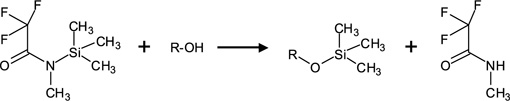
\includegraphics[width=0.8\textwidth,natwidth=4.17in,natheight=3.32in]{./Figures/silylation.jpg}
	\rule{35em}{0.5pt}
	\caption[A silylation reactio]{The silylation reaction to facilitate the chromatography of glycerides.}
	\label{fig:Silylation}
\end{figure}

\section{\texorpdfstring{\GCxGC}{GCxGC}}

Comprehensively coupled \GCxGC has been used to analyse biodiesel.

\section{SFC}

Supercritical fluid chromatograpy was invented by Klesper e.a. in 1962 \cite{} using CFCs, altough the first mention of the phrase `supercritical fluid' found by the indexing service Scopus is a paper by Sie and Rinders in 1967, who used carbon dioxide. According to Saito (one of the oldest workers in this field) \cite{Saito2013} or cite (jp.linkedin.com/pub/muneo-saito/17/500/30) it developed somewhat, but in the 1980s capillary column supercritical fluid chromatography appeared and was oversold, which confused users about the use and potentials of SFC. During the 1990s some applications for SFC appeared, and it found a solid niche in the pharmaceutical industry.

First work experimented with various substances (SF6) above their supercritical points, but the low price, inertnes, non-toxicity and reasonable critical point (37 degC at 7.38MPa) made carbon dioxide the universal mobile phase for SFC today. 

SFC with FID detection had the wonderful feature that it was a universal mass sensitive detector.

SFC with MS: what are the problems. Solvable with GC very well known. 

We are much encouraged by the introduction or commercial instrumentation, such as the Waters UPC2 system. 

\section{LC}

According to the review of Pauls \cite{Pauls2011} LC methods for the analysis of biodiesel are growing and "liquid chromatographic methods are beginning to gain favor and are likely to become more widely utilized with improvements in detector technology." 

Of particular interest to our work are the normal phase LC procedures reported. As a rough rule of thumb, supercritcal carbon dioxide has the solubility of dichloromethane, so that using supercritical carbon dioxide with a silica column is approximately like doing normal phase liquid chromatography. 

The use of silver ions in stationary phases to separate 

\section{HPLC-GC}



\section{Miscellaneous}	

In the early enthusiasm for biodiesel much was said about the benefit that biodiesel could have for countries and regions with little money but agricultural potential. If one assumes that biodiesel would be produced locally and not the oil simply exported, the question arises about what one can do about quality control without expensive LC and/or GC equipment. One answer is the use of more traditioal methods of wet chemsitry. Pisarello \cite{Pisarello2010} suggests a titrimetric method, which requires no expensive instrumentation. An examination of the citing papers show that, eight of the nineciting papers were in the field of biodiesel production. The exception was a review paper. 

\section{Techniques similar to \SFCxGC}
	\subsection{SFC-GC}
	Fractions of SFC can be collected. 
	\subsection{\SFCxSFC}
	The Japanese used SFCxSFC to analyze trigycerides \cite{Hirata2003}and FAMEs \cite{Hirata2004} using \SFCxSFC.  % Literature Background

% Chapter 3

\chapter{Instrumentation: Fast Temperature Program GC} % Write in your own chapter title
\label{Chapter3}
\lhead{Chapter 3. \emph{Fast GC}} % Write in your own chapter title to set the page header

\section{The nature of the problem}

Before we look at the experimental work, it would be useful to put the research problem into the context of problems in general. I will be using Ulrich's \cite{Ulrich2011} taxonomy. (Figure~\ref{fig:ProblemTaxonomy})

\begin{figure}[htbp]
	\centering
	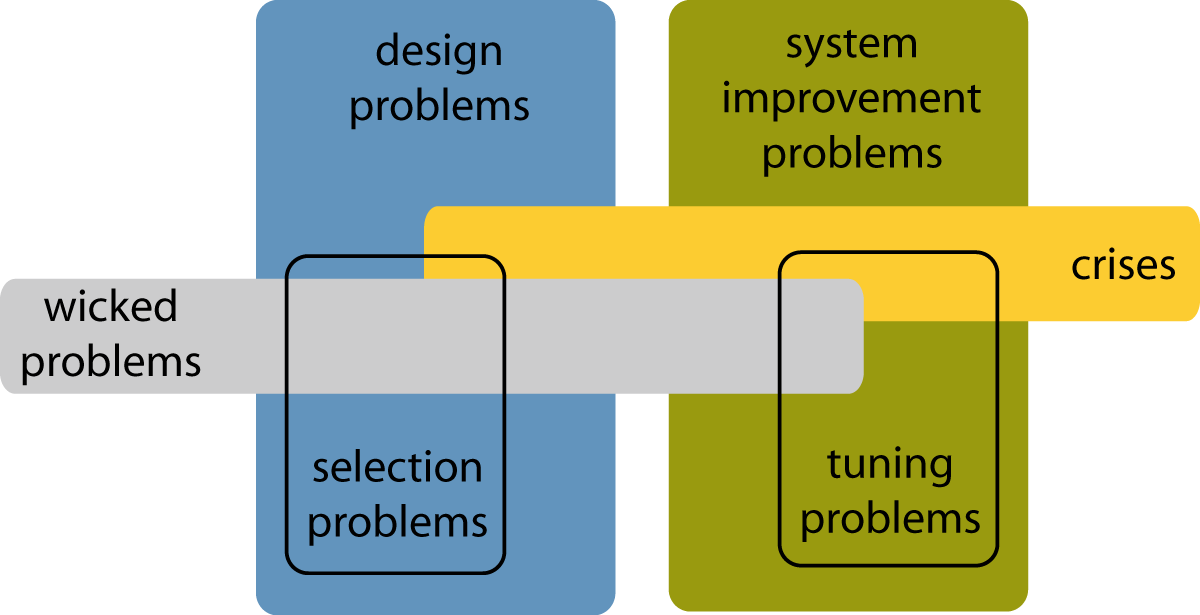
\includegraphics[width=0.8\textwidth,natwidth=4.17in,natheight=3.32in]{./Figures/ProblemTaxonomy}
	\rule{35em}{0.5pt}
	\caption[Taxonomy of Problems]{A simple taxonomy of problems}
	\label{fig:ProblemTaxonomy}
\end{figure}

Not every research problem will, in the end, contain a design problem. In terms of analytical chemistry, say a system improvement problem such as needing to improve resolution between critical peaks, may easily be solved by simply optimizing the chromatography, making it a tuning problem. But it might also be that the system improvement (increasing resolution) will demand a new stationary phase. This then becomes a selection problem, a subste of design problems. 

Many chromatographic problems are system improvement problems, or selection problem. Method development in GC is typically a selection problem: select stationary phase, select flow rates and temperature programmes. Often the design problems of analytical chemistry lies in sampling and sample preparation

In developing our system, we were faced by a true design problem, in at least three dimensions: mechanical, software/electronics, and chromatographic. 

\section{Why fast temperature program gas chromatography?}

The use of temperature programming for GC in \SFCxGC is required by the wide range of boiling points expected in the second dimension. Otherwise the general elution problem will cause the spreading out of peaks of high-boiling compounds, or the loss of resolution of low-boiling peaks, depending on the temperature 

Fast temperature programming is desirable because of the expected duration of the \SFCxGC run. 

$t_{total} = t_{SFC total} + \frac{t_{SFC total}}{t_{SFC fraction}} \times t_{GC run}$

If a typical SFC run takes 20 minutes, and fractions are collected for every 5 seconds of SFC run, it means there will be 20*60/5 = 240 fractions collected. Each of these must become a GC run. If each GC run took a minute, the \SFCxGC run would last 4 hours. This is not unheard of in chromatography, but \GCxGC runs take as long as the first dimension run, so \SFCxGC would not compete in terms of time

Obviously the $t_{SFC fraction}$ can be increased for a smaller $t_{total}$ but too large an SFC fraction can overload the GC column.

\section{Fast GC theory}

A specific separation problem needs a certain number of theoretical plates, $N_{req}$. In fast chromatography the question is how this number of plates can be achieved in the shortest time. 

\begin{equation}
t_r = (1+k) N_{req}^\frac{3}{2}\frac{9}{8}\sqrt{3}F(k)\left[\frac{\eta}{p_0 D_{m,o}}\right]^\frac{1}{2}d_cS2T
\label{eqn:tr}
\end{equation}

For a a

\begin{equation} 
N_{req}= 16R^2_s\left[\frac{1+k}{k}\right]^2\left[\frac{\alpha}{\alpha-1}\right]^2
\label{eqn:Nreq}
\end{equation}

\begin{equation}
F(k) = frac{1+6k+11k^2}{96(1+k)^2}
\label{eqn:EquationLabel}
\end{equation}

\begin{figure}[htbp]
	\centering
	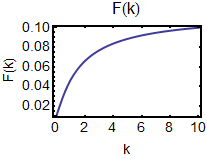
\includegraphics[width=0.8\textwidth,natwidth=4.17in,natheight=3.32in]{./Figures/F(k).png}
	\rule{35em}{0.5pt}
	\caption[Dependence of F on k]{Dependence of F on k}
	\label{fig:F(k)}
\end{figure}

Figure~\ref{fig:F(k)} shows the dependence of $F$ on $k$. This shows that lower k gives smaller F. This is in keeping with the $(1+k)$ term, so that there is no minimum $t_r$ dictated by $k$.

Examining Equation~\ref{eqn:tr} it becomes apparent that to minimize $t_r$ one can reduce $N_{req}$ or the last two terms. 

$N_req$ can be reduced by minimizing the resolution to the lowest sufficient value. This means leaving some peaks unresolved. 

Reducing the resolution can be achieved by: 
\begin{itemize}
	\item using a shorter column
	\item using a higher gas flow 
	\item using a higher temperature
	\item using temperature programming
	\item using pressure or flow programming
	\item using a thinner film
\end{itemize}

Improving the selectivity ($\alpha$) will also reduce the number of plates needed. This can be improved by:
\begin{itemize}
	\item selecting a different stationary phase
	\item using selective detection, for example an electron capture detector.
	\item using MS detection.
\end{itemize}


Further

%The Van Deemter curve predicts the optimum HETP. There is no way of improving the resolution. In general, doing faster GC, using shorter columns and increasing the mobile phase flow will lead to poorer resolution. However, if the peak density can be reduced, there might be surplus resolution, and the speed of the separation can be improved. The surplus resolution can be generated either on the detector side, or on the sample side.

%On the detector side, surplus resoluton can be generated by selective detection, such as 

%On the sample side, surplus resolution can be 



\section{How the temperature measurement works}

Consider two resistors in series $R_{col}$ and $R_{ref}$, with $R_{col} \gg R_{ref}$. $R_{col}$ represents the resistance of the column, and $R_{ref}$ represents the resistance of the reference column. Because of the resistance ratio most of the heat developed in the circuit is developed in $R_{col}$. 

The circuit is supplied by a voltage $V_{sup}$, in general an unknown value. $V_{col}$ and $V_{ref}$ represents the voltage drop over the respective resistors. 

Because the current $I$ through the circuit is the same for both $R_{col}$ and $R_{ref}$, it is true that $\frac{R_{col}}{V_{col}}=\frac{R_{ref}}{V_{ref}}$, and therefore \begin{equation}R_{col} = R_{ref}\frac{V_{col}}{V_{ref}} \end{equation}

The voltage drop across $V_{ref}$ is small, and therefore it is amplified by the amplifier with gain $g$, so that $V_b = gV_{ref}$

$V_{sup} = V_{col} + V_{ref}$ 

$V_{sup}=dV + V_b$

$V_{col} + V_{ref} = dV + V_b$

$V_{col} + V_{ref} = dV + gV_{ref}$

$V_{col} = dV + gV_{ref} - V_{ref} $

$V_{col} = dV + V_{ref}(g - 1)$

$\frac{\displaystyle V_{col}}{\displaystyle gV_{ref}} = dV/gV_{ref} + V_{ref}(g-1)/gV_{ref}$

$\frac{\displaystyle V_{col}}{\displaystyle V_{ref}} = gdV/gV_{ref} + gV_{ref}(g-1)/gV_{ref}$

$\frac{\displaystyle V_{col}}{\displaystyle V_{ref}} = gdV/V_b + (g-1)$

This proves that $\frac{\displaystyle V_{col}}{\displaystyle V_{ref}}$ is a linear function of $dV/V_b$. A quick check for correctness of the expression: for a unity-gain amplifier $g = 1$, and $\frac{\displaystyle V_{col}}{\displaystyle V_{ref}} = dV/V_b$.


\subsection{Assumptions}

The assumption is that the temperature is a function of the resistance of the column, or $T = f(R_{col})$. Because $R_{col}=m(^{dV}/_{V_b}) + c$, we can say that $T = f'(^{dV}/_{V_b})$. Through a calibration procedure $f'$ can be approximated by a polynomial. 

\section{Calibrating the Column}

The calibration of coaxial heater. 

\subsection{Thermocouple}

The problems of measuring a temperature inside a tube with a bore of 1 mm is not trivial.

The following methods can be used to measure temperatures.
\begin{itemize}
	\item Liquid-in-glass thermometers
	\item Sealed liquid or gas sensing instruments and bimetallic sensors.
	\item Electrical Resistance Temperature measurement using metallic sensors
	\item Thermistors and semiconductors
	\item Thermoelectric temperature measurement
	\item Disappearing filament optical pyrometer
	\item Photoelectrical optical pyrometers
	\item Total radiation pyrometers.
\end{itemize}

Liquid-in-glass thermometry would not be applicable because of the size of the devices, and because they don't give a desirable electrical signal. Radiant energy methods would not be of much use at the lower end of the temperature range, and will also only measure the outside wall surface temperature of the heater. This leaves us with resistance temperature measurement with metallic sensors, thermistors and semiconductors, and thermoelectric.

Thermistor and semiconductor devices could, in principle be made small enough for the job, but affordable packages are too large. Besides that, the operating temperature range is a bit extreme for semiconductors that generally have an upper temperature limit of about 200 (?) �C. 

Electrical resistance measurement using metallic sensors are quite feasible, if a sensing element of the right dimensions are available. These are not easy to find. Additionally, because long thin wires would be needed to connect the sensing element to the electronics.

Thermoelectric temperature measurement then remains. This uses the effect that a circuit of two dissimilar metals will generate a voltage when there is a temperature gradient along the conductors. The voltage generated is a function of the temperature difference between the junctions of the two metals. Thermocouples are widely used in industry for measuring temperatures, and the technology is well established. Thermocouple wire can be purchased in varying gauges, down to 25 $\mu$ m in diameter. 

McGee \citep{Mcgee1988} states that thermocouple junctions can be made by welding, crimping, soft soldering, hard soldering, bolting, or simply twisting the wires together.

Because of the temperature range expected to be measured (-50�C to 350�C) the option of soft soldering does not apply. Because of the possibility of corrosion, bolting or twisting the wires together are not good options.

This leaves welding, crimping and hard soldering. The option of crimping was not explored, chiefly because the author has no knowledge of the technology or of any devices that could do this. Two patents (ref?) (ref?) available on the topic shows another problem: the final crimped connection has a diameter many times the diameter of the wire. This precludes the application of crimping in this context.

How the thermocouple probe was made:

\begin{enumerate}
	\item A piece of 0.25 mm polyimide-coated fused-silica capillary of about 500 mm length was cut and mounted with sticky tape on a wooden metre stick.
	\item A longer length of 0.1 mm fused-silica capillary was threaded through the 0.25 mm capillary.
	\item The end of one of the thermocouple wires was inserted into the end of the 0.1 mm capillary. A drop of cyanoacrylate adhesive was touched to the end of the capillary. Capillary action drew the liquid adhesive into the capillary and fixed the wire in place.
	\item The wire was drawn carefully into the capillary by pulling on the 0.1 mm capillary.
	\item Once the end of the wire protruded through the end of the 0.25 mm capillary the end of the 0.1 mm capillary was cut off.
	\item The wire was anchored at one end with adhesive tape, pulled tight, and anchored at the other end. 
	\item The procedure was repeated for the other wire.
	\item The two thermocouple wires (Goodfellow) was clamped in a twisting bar. The twister bar has a square profile, 8 mm on a side.
	\item The wires were flamed with a cigar lighter until they were red a dull red hot. (At any higher temperature the wires would melt.) This chars the polyimide coating.
	\item The flamed portion of the wires were lightly sanded with 1200 grit water paper. A pair of small pliers had its beak lined with the abrasive, and lightly stroked up and down the wire to remove the char.
	\item A 6 mm tube was inserted between the wires to serve as spacer. and moved until about 10mm away from the twister bar.
	\item The wires were twisted by turning the twister bar until the twister portion was about 5mm long.
	\item The spools were rewound to retract the wire, until the start of the twist rested on the clamping bar.
	\item The clamping weight was lowered onto the clamping bar, keeping the pair or wires in place.
	\item A small pair of scissors was used to snip off the end of the
	\item The welding electrode was brought into position. This was a carbon rod in the form of a pencil lead (Schwann Stabilo), 2 mm in diameter, mounted on a screwing connector. The welding circuit consisted of a bench power supply set to approximately 20V. connected. The negative terminal was clamped to the aluminium base plate of the microscope, on which rested the brass clamp bar. The positive terminal was clamped to the carbon electrode. A voltage of approximately 23 V was applied.
	\item It was discovered that the carbon electrode should not have a polished end, but a roughly broken end. 
	\item The electrode was moved closer to the clamped twisted wire.
	\item At the right point a spark would jump from the carbon to the wire, melting the end of the wire. The molten wire would draw into a globule on the end of the wire, withdrawing from the electrode and so breaking the spark, ending the heating.
	\item If the wire would actually touch the electrode the wire would heat up red hot and melt off, usually destroying the twist and requiring making a new twist.
	\item If all went well, there would be a hemispherical weld at the end of the twist where the two wires would be joined.
	\item The thermocouple wires was withdrawn into the capillary until the end just protruded, kept in place with a pair of rubber-tipped self-closing tweezers.
	\item If two sets of thermocouples were needed, the procedure would be repeated for another pair of wires.
	\item The wires would be pulled back, one pair at a time.
	\item The other end of the capillary was taped to the connector pad.
	\item The wires was flamed and scraped to remove the polyimide isolation, and screwed down on a screw connector block.
	\item The resistance between the protruding end of the thermocouple and the connector block was measured to ensure electrical connection. The resistance for the Chromel is 1440 $\Omega{m}^{-1}$, and for the Alumel 600 $\Omega{m}^{-1}$
\end{enumerate}

\section{Thermocouple Welding}

\begin{figure}[htbp]
	\centering
	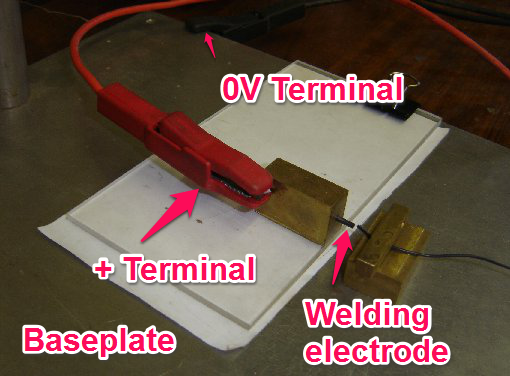
\includegraphics[width=0.8\textwidth,natwidth=4.17in,natheight=3.32in]{./Figures/Welder.png}
	\rule{35em}{0.5pt}
	\caption[Fine-wire welder]{A view of the fine-wire thermocouple welder.}
	\label{fig:Welder}
\end{figure}

\begin{figure}[htbp]
	\centering
	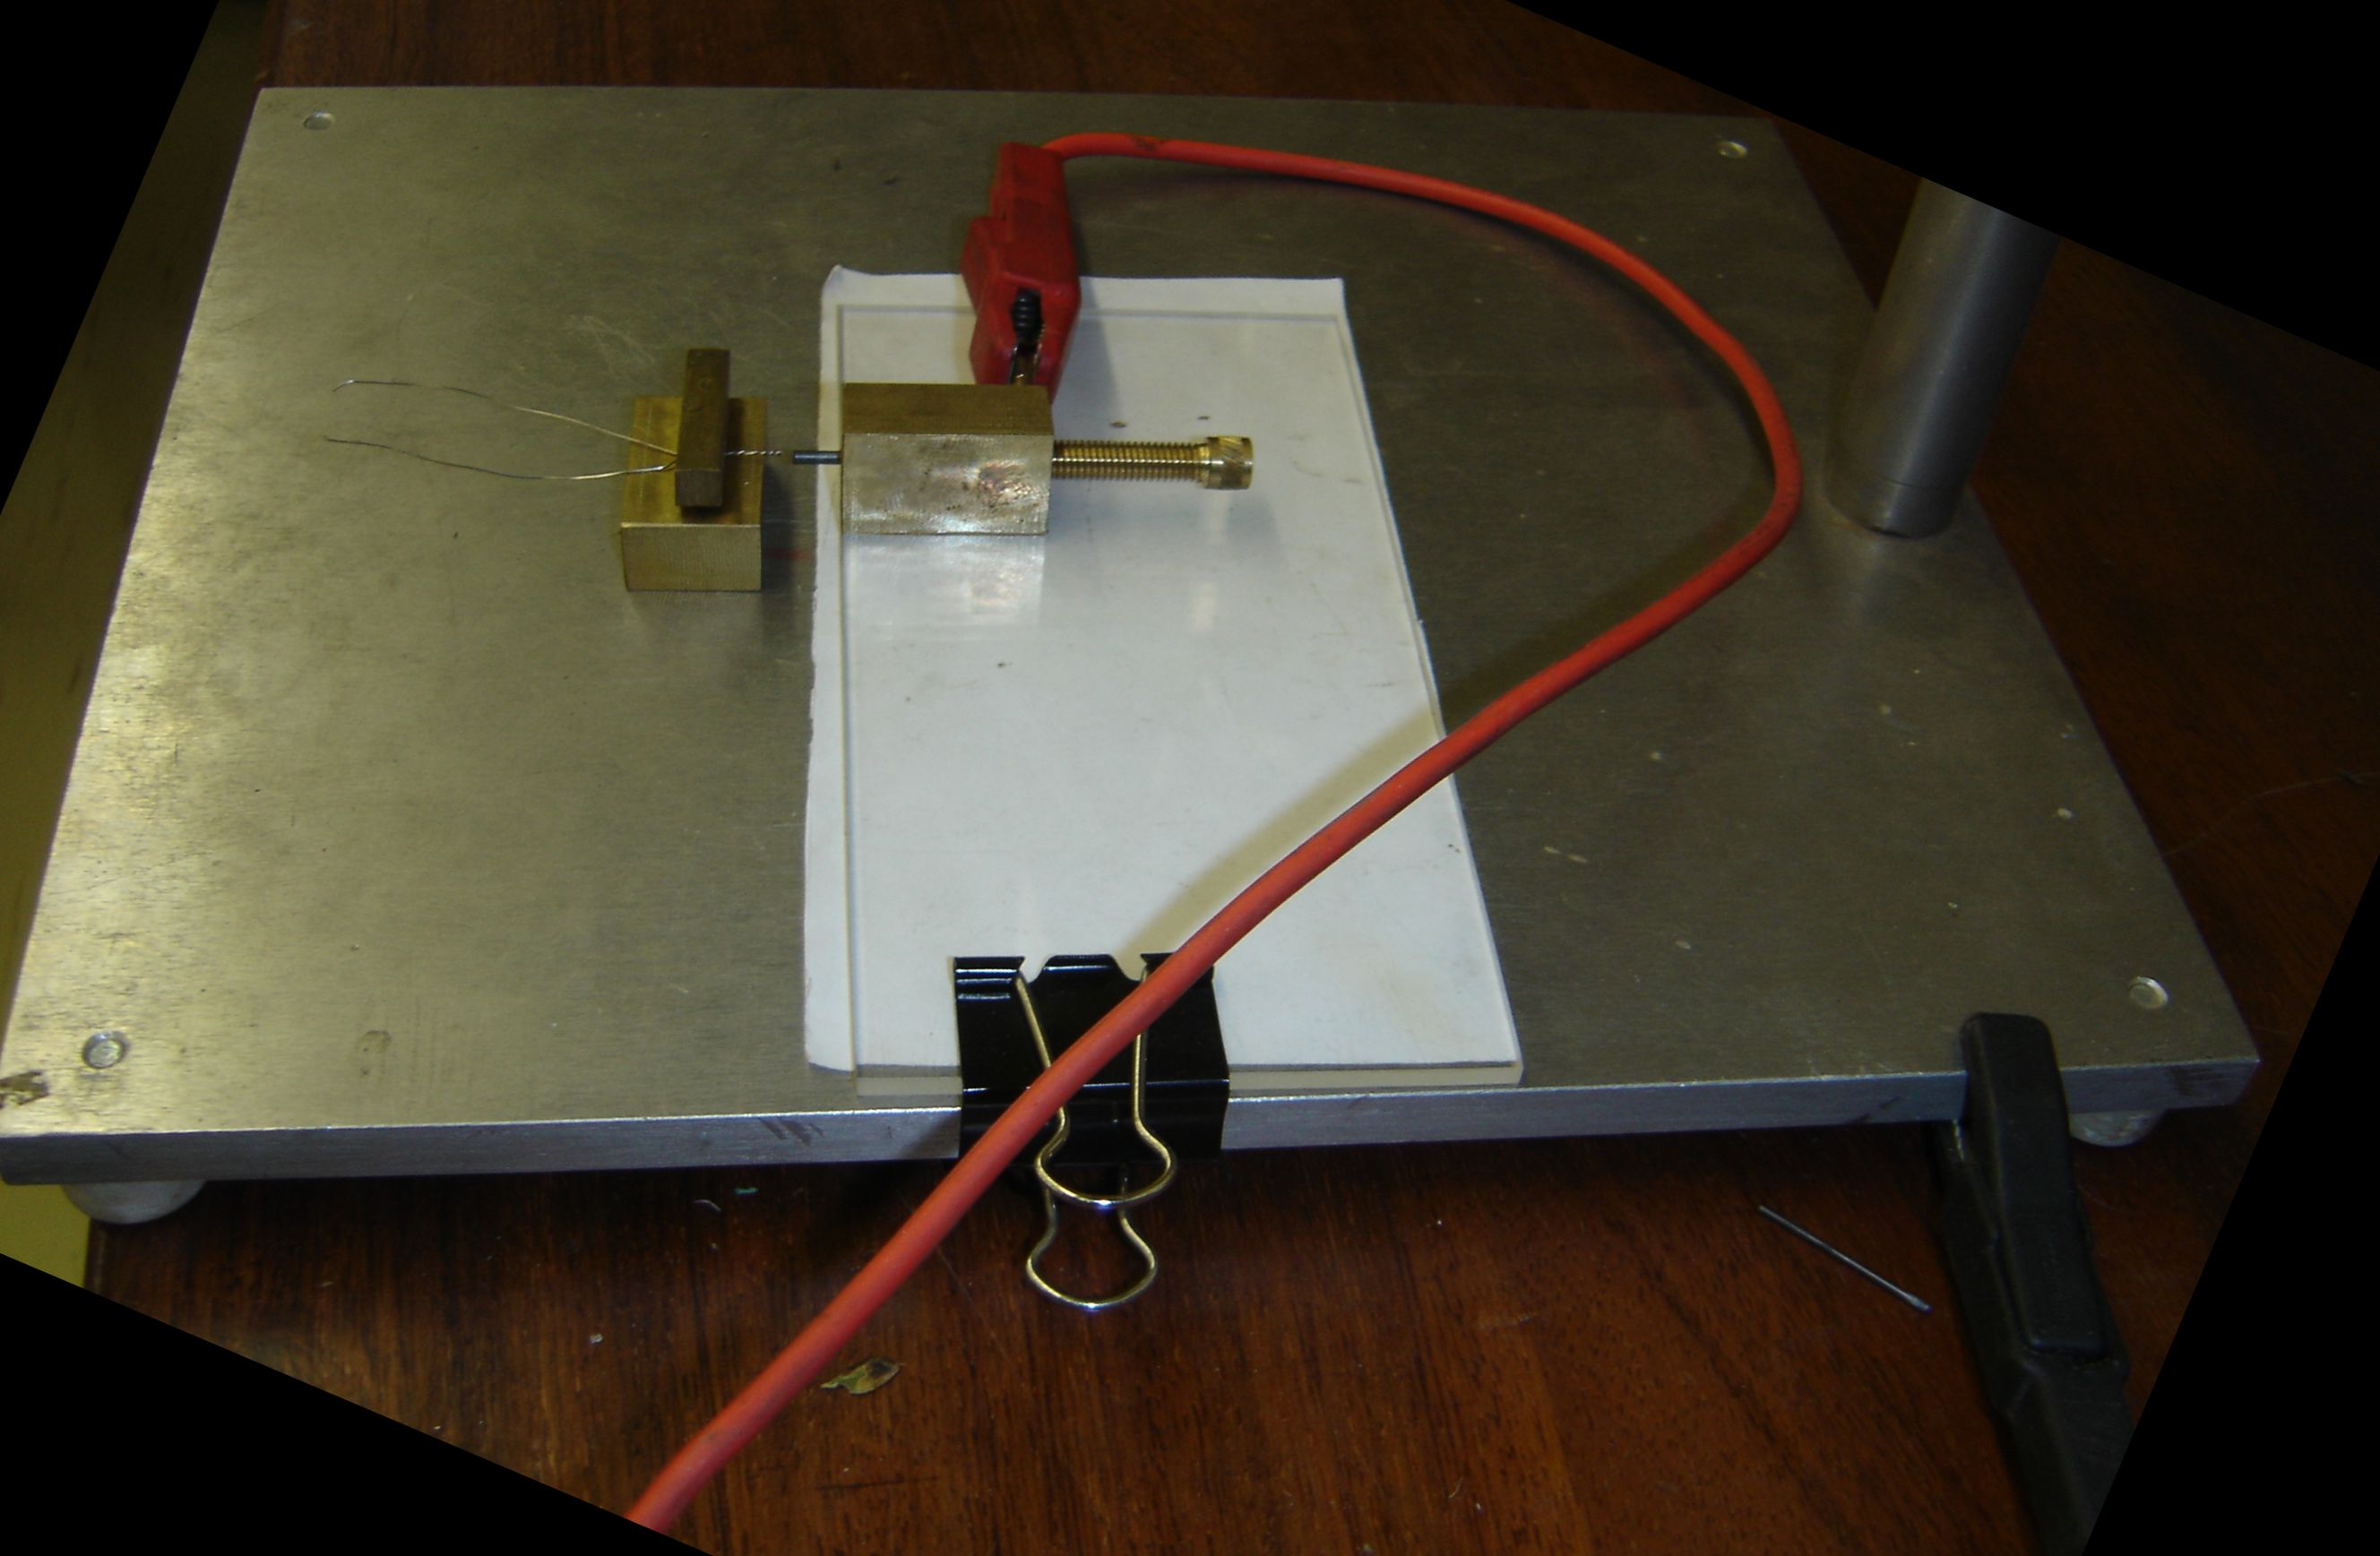
\includegraphics[width=0.8\textwidth,natwidth=4.17in,natheight=3.32in]{./Figures/Welder2.jpg}
	\rule{35em}{0.5pt}
	\caption[Fine-wire welder]{A view of the fine-wire thermocouple welder. The wire shown is much thicker than that actually used. It is shown clamped between the clamping bar and the clamping weight. A thin sheet of Perspex serves to isolate the positive electrode from the negative base. The carbon electrode can be advanced towards the thermocouple twist using the screw. The black clamp at the bottom right-hand corner attached to the base plate and the red clamp attached to the screw housing provide a potential difference of approximately 20 V between the carbon electrode and the thermocouple.}
	\label{fig:Welder2}
\end{figure}


\begin{figure}[htbp]
	\centering
	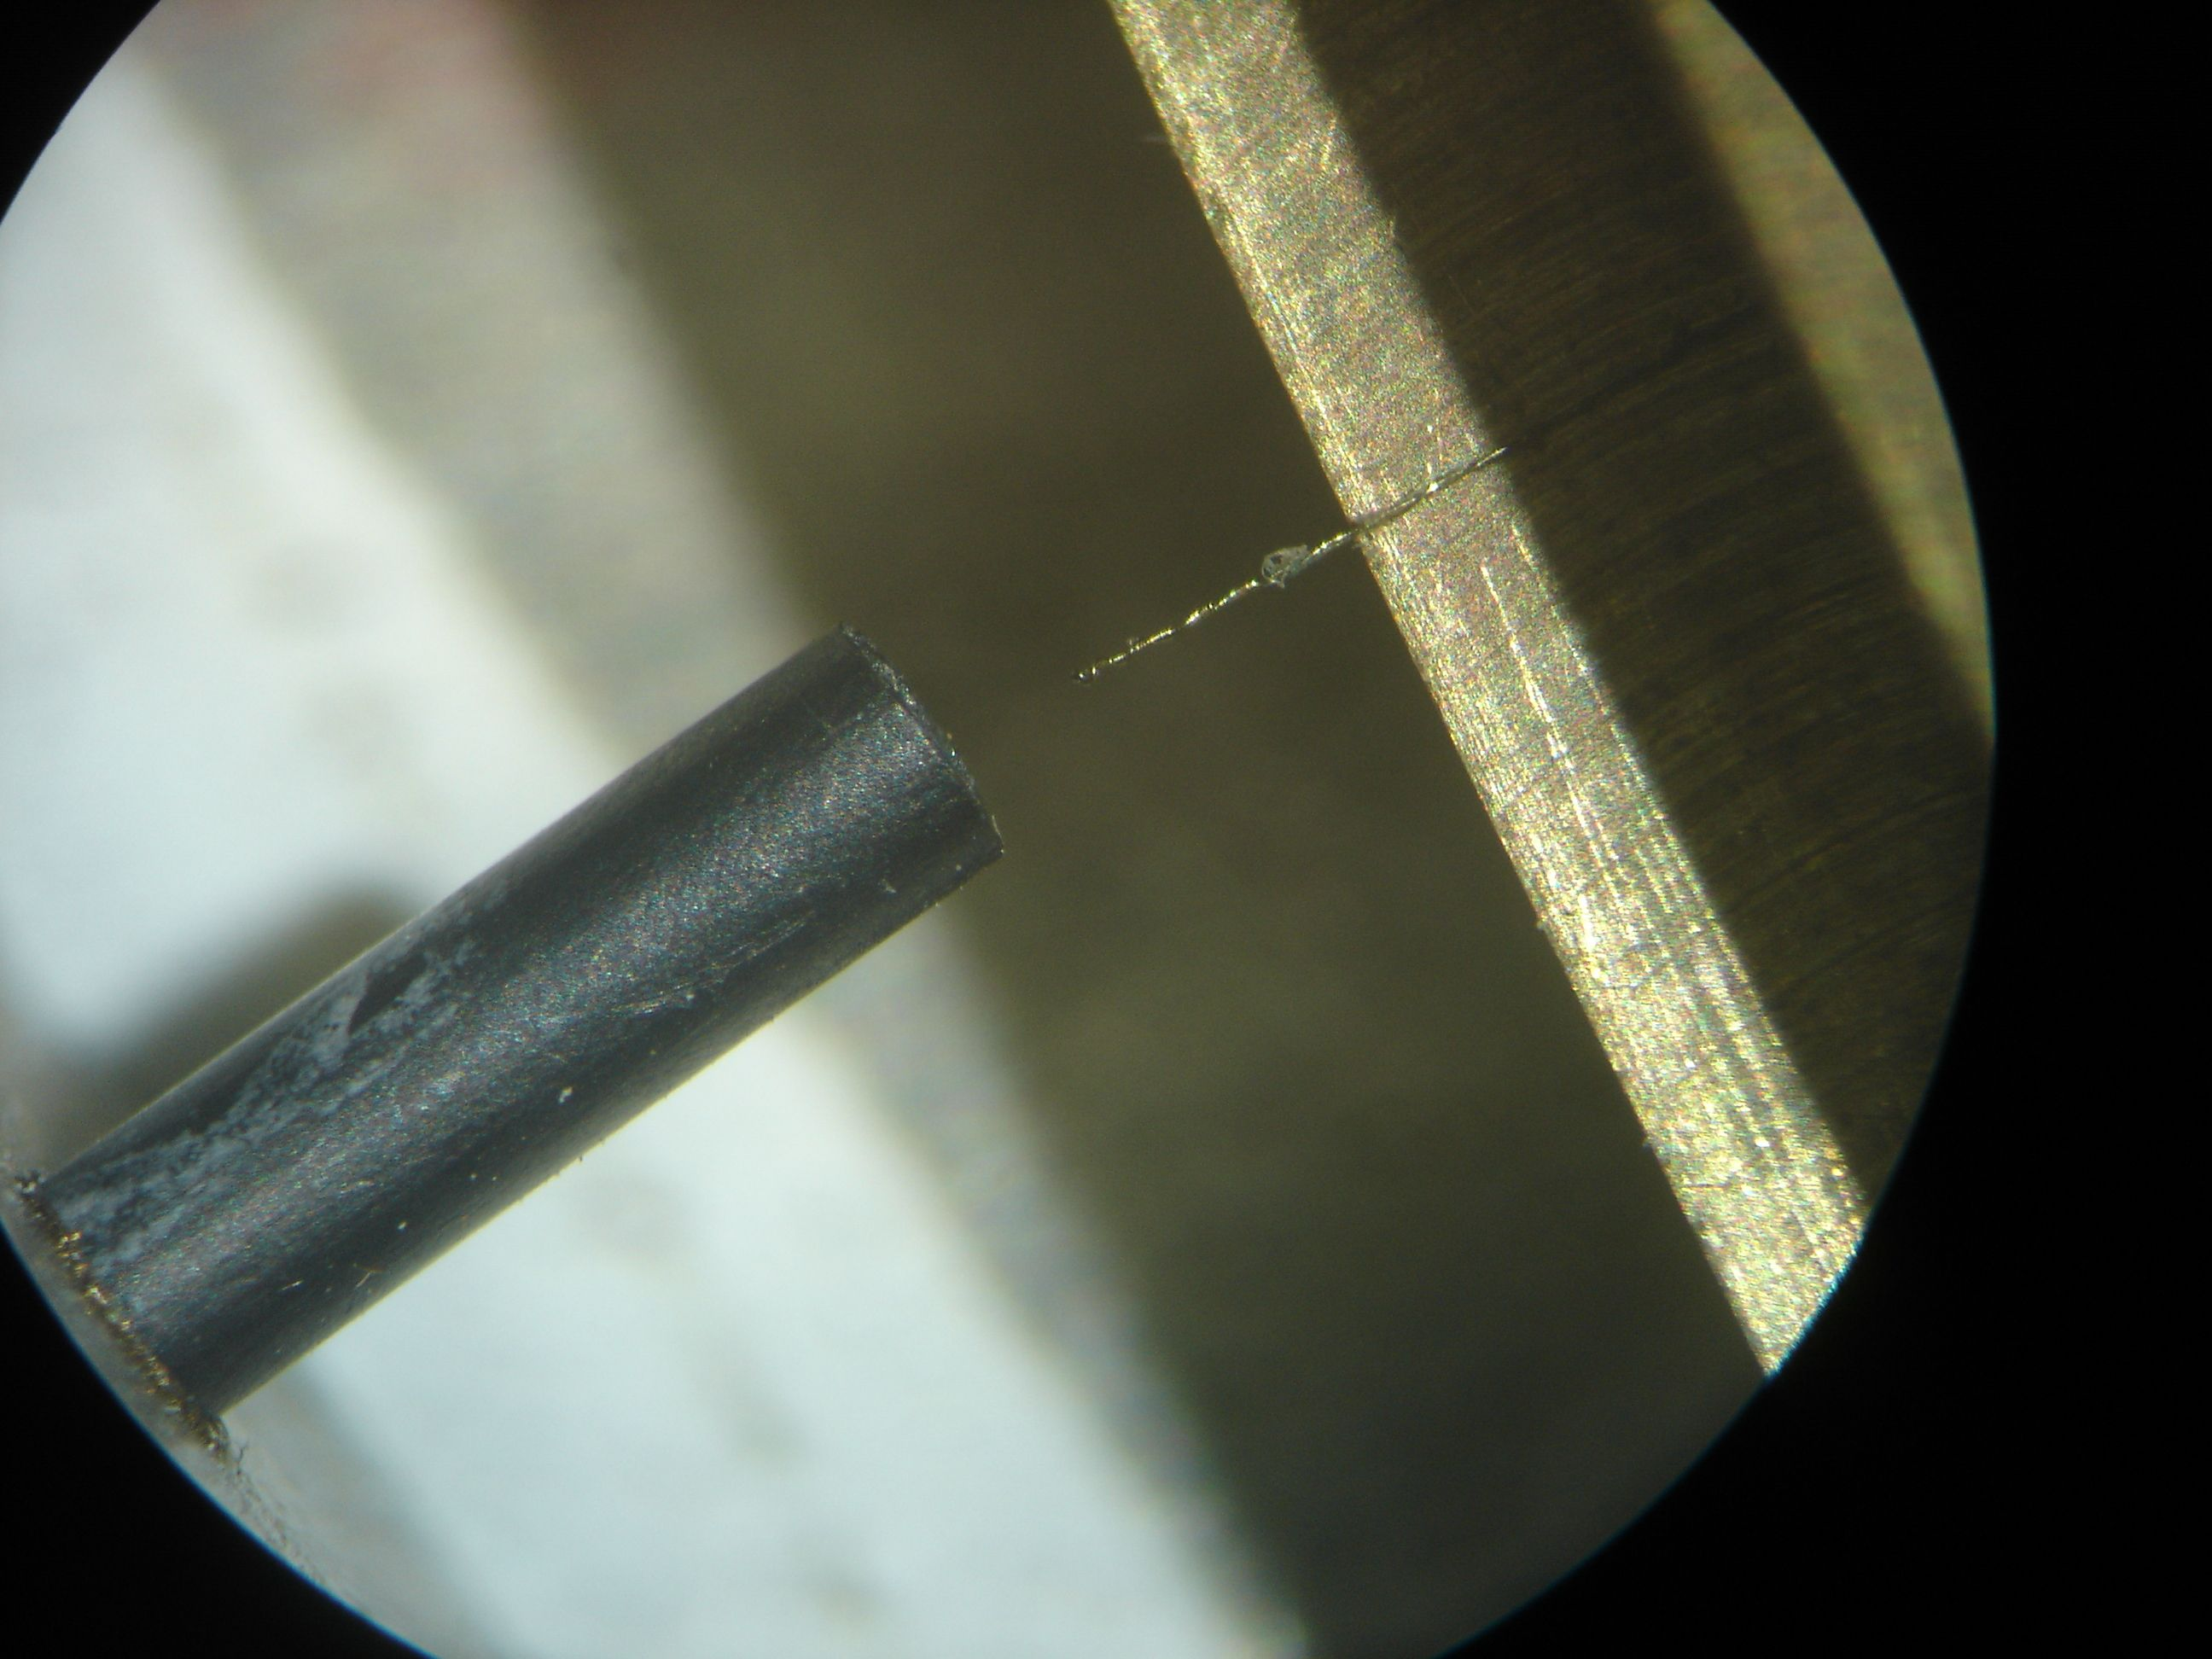
\includegraphics[width=0.8\textwidth,natwidth=4.17in,natheight=3.32in]{./Figures/WelderMicro.jpg}
	\rule{35em}{0.5pt}
	\caption[A microphoto of a thermocouple twist ready to be welded.]{A microphoto of a twisted wire ready to be welded. The black carbon electrode is 2mm in diameter.}
	\label{fig:TheFigureLabel}
\end{figure}


\section{Extra} % Instrumentation: Fast GC

% Chapter 4

\chapter{Instrumentation: Gradient elution SFC} % Write in your own chapter title
\label{Chapter4}
\lhead{Chapter 4. \emph{Gradient SFC}} % Write in your own chapter title to set the page header

\section{Supercritical Fluid Chromatography}

The source of high-pressure carbon dioxide for SFC was high-purity carbon dioxide from Air Products. Carbon Dioxide 4.5, meaning carbon dioxide that is 99.995\% pure. 

At 5.6 MPa the pressure is not near the supercritical range. It is a mere 55.3 atm, while we do the supercritical chromatography at 200 atm. The critical pressure of carbon dioxide is 7.39 MPa. At 200 atm, which translates to 20.27 MPa, there is 

We work at below the critical temperature of carbon dioxide, (an easy-to-remember 300K, or 37�C), but by using such a high pressure it means that the gas is overwhelmingly in the liquid phase.

(It is widely recognized in the field now that SFC has become a misnomer. SCF is not usually done above the critical temperature, and sometimes at quite modest pressures. At Pittcon 2010 I heard someone refer to it as `Separation Facilitated by Carbon dioxide'.)

\begin{figure}[htbp]
	\centering
	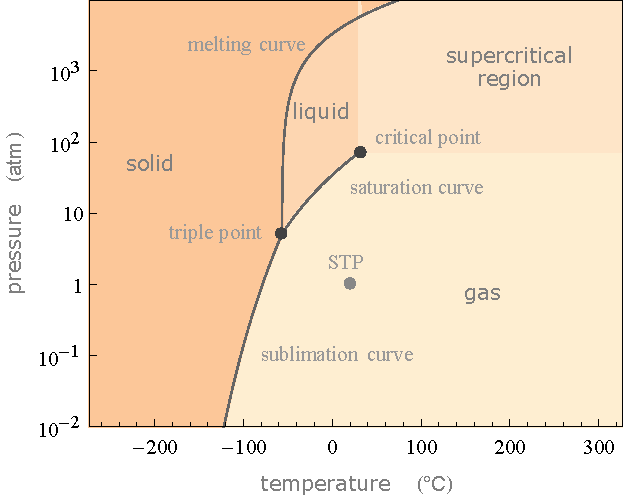
\includegraphics[width=0.8\textwidth,natwidth=4.17in,natheight=3.32in]{./Figures/CO2pVdiagram.pdf}
	\rule{35em}{0.5pt}
	\caption[Phase diagram]{The phase diagram for carbon dioxide}
	\label{fig:PhaseDiagram}
\end{figure}

\section{SFC}
%Varian 8500 LC pump.
%Pressure guage

The liquid carbon dioxide from the cylinder was conducted to the Varian 8500 LC pump.

Although the pump's `Fill' was used to fill the empty cylinder, this should not create the impression that the pump aspirates the liquid carbon dioxide from the bottle. The moment the carbon dioxide enters the pump cylinder, the vapour pressure will be determined by the temperature. While the pump can produce a small amount of underpressure, the vapour pressure will dominate. Therefore a hot pump cylinder will not fill with liquid, because the pressure inside the cylinder will press any liquid back into the dip tube, and the pump will only fill with vapour. The pump needs to be cooled to allow the liquid into the cylinder. 

At 200 atm the pump leaks at xxx nl/s

A chiller from Labotec with a 20 l capacity was filled with a solution of 7.5 l of diethyl glycerol and 7.5 l of water. This mixture has a freezing point of -10 deg C, which can be cooled by the chiller without freezing. (If the coolant freezes a hump of ice forms on the cooling plate of the chiller, which isolates the remaining liquid and limits the temperature of the coolant to the melting point of the coolant.)

Unfortunately the higher viscosity of the mixture compared to water makes it more difficult to pump reducing the pump `head' of the Labotec stirrer/heater/pump so much that it couldn't pump the liquid from the chiller on the floor to the top of the pump cylinder, preventing the circulation of coolant. Therefore an inexpensive submersible WH1200 water pump from Waterhouse was acquired, which can deliver 800 l of water per hour at a head of 1.2m.

We also used a SFT-10 pump from Supercritical Fluid Technologies (Newark, Delaware). This is a purpose-built two-piston pump with a sapphire pistons and a Peltier-cooled head. This is a much better technology than the HPLC pumps. It takes up less space and does not need refilling, since it feeds directly from the cylinder. 

\section{Gradient Elution SFC}

\subsection{Pressure Programming}

In the early days of SFC the solubility of the mobile phase was tuned by adjusting the pressure. Using this adjustability one could obtain gradient elutions by simply adjusting the pressure of the mobile phase.

\subsection{Modifier Programming}
It was soon realized that this tuning range is not particularly wide, and pretty soon people were adding modifiers to the carbon dioxide. Adding a modifier makes dramatic differences to the dissolving power of the carbon dioxide, but reduces the compressibility. This means that varying modifier concentration has replaced pressure tuning as the primary means of gradient elution in SFC. 

We made provision for addition of a single modifier to the carbon dioxide. The SFC system operated under constant pressure, but it was easy to calculate the flow provided by counting the number of steps given by the stepper motor of the pump to maintain that pressure. Before the column we had a six-port valve configured with a injector loop. This loop was filled with methanol from a second HPLC syringe pump. The volume of this loop was determined colourimetrically. By regularly switching the modifier valve the contents of the injection loop is placed in the mobile phase and the selected concentration achieved.

This approach is not without its problems. When the valve switches from ``Inject'' back to ``Load'', the liquid carbon dioxide in the injection loop is exposed to the atmosphere and it expands explosively. Rather unexpectedly, it expands into the methanol supply line, blowing a part of the methanol in it out. (A tentative explanation for this that the high pressure gradient drives bubbles of carbon dioxide gas into the supply tube. As these bubbles expand when the pressure drops, it forces the methanol from the tube.) This emptying of the methanol tube means that the methanol consumption is much higher than one would expect. In the case of using toxic or irritant modifiers one would need a means of extracting the vapours.

Care has to be taken to ensure that the mixing downstream of the valve is adequate, otherwise an oscillating modifier concentration will be result.

%graph of measurement of loop volume?

\subsection{Additive Programming}

Additives are minor compounds that are added to the mobile phase to 

\section{Restrictors}

In HPLC and UPLC, the most common detectors are UV detectors that use pressurized flow cells. After the detector there is a back-pressure controller that controls the pressure in the chromatographic system.

\begin{quote}
Changes in pressure can greatly vary the characteristics of SFC. Achieving extraction and chromatograms with high reproducibility on a supercritical fluid system requires a device that can perform pressure control in a stable manner. JASCO offers the BP-2080, which is capable of automatic pressure control, and the BP-2080-M, which is capable of manual pressure control.
BP-2080/2080-M Back Pressure Regulator

The BP-2080 and BP-2080-M employ a patented flow-switching valve (FSV) mechanism that enables stable system pressure control even at the lowest volume limit possible. The FSV mechanism regulates pressure by controlling the channel opening while a needle vibrates at a high rate of speed. This prevents blockages due to high-viscosity elution samples and solidified samples, which can be a problem with static pressure regulators. This enables stable system pressure, even during long-term continuous operation. Since the BP-2080 has a time program feature that can control pressure and temperature according to the passage of time, it makes it easy to automate analysis work. The BP-2080M offers manual control for the volume passing through the opening in the FSV mechanism.

\end{quote}

In the case of restrictors there is too little we can do.

The restrictor has a two-fold function. \begin{enumerate}
	\item It controls the flow of the eluent from the column. If there is no flow, the pressure difference over the column is zero, and there is no flow. By opening an orifice in the form of a restrictor, there is a flow of eluent from the column, reducing the outlet pressure, thus allowing flow through the column. The size of the orifice controls the pressure at the column outlet, and thereby the chromatographic flow. 
	\item It maintains the pressure inside the chromatographic column at supercritical pressure. 
\end{enumerate}

The restrictor can be of different designs. 

As a first approximation we can use the Hagen-Poiseuille equation

\begin{equation}
Q = \frac{\pi R^4}{8\mu}\frac{\Delta p}{L} 
\label{eqn:Hagen-Poiseuille}
\end{equation}

This is of course only a very rough approxmation, because we are using a compressible, condensing fluid with the temperature dropping quickly because of adiabati expansion. But it will serve to illustrate different approaches.

The linear restrictor uses the pressure drop over the lenght of a straight piece of capillary. This increases $L$, which, for a given length. 

With the integral, or micro-hole, restrictor, the radius of a short length of pipe is controlled. Because of the fourth power, a small increase in radius allows a much greater pressure drop.

The third design, the frit restrictor, uses a combination of small holes and length. The length is the controlled factor.

\begin{description}
	\item[Linear restrictor] The linear restrictor is merely a long piece of 
	\item[Orifice restrictor]
	\item[Frit restrictor] D
\end{description}

We used the `integral' restrictor as described by Guthrie and Schwartz. We've had good experience with these models. It uses only a small amount of capillary column, and gives a good degree of adjustibility, for a fairly simple procedure. The percieved benefit of this design was that it would not cause discrimination by the lenghty pressure drop. 

But in practice we discovered that micro-orifice restrictors blocked. At first it was assumed that it was particles from the stop-flow valve that were blocking the orifice, and we installed a half-micron filter. (Univerversal Mini Filter, 0.5 $\mu$m, Grace, Deerfield Illionois. The restrictor plugging was unpredictable and irregular. To determine the cause of the plugging, , a number of plugged restrictors were prepared for scanning electron microscopy (SEM). 

In many cases there were no plugging visible, but the restrictor still stopped flow. 

To from an idea of what to expect we first examined a blank piece of capillary. 

\begin{figure}[htbp]
	\centering
	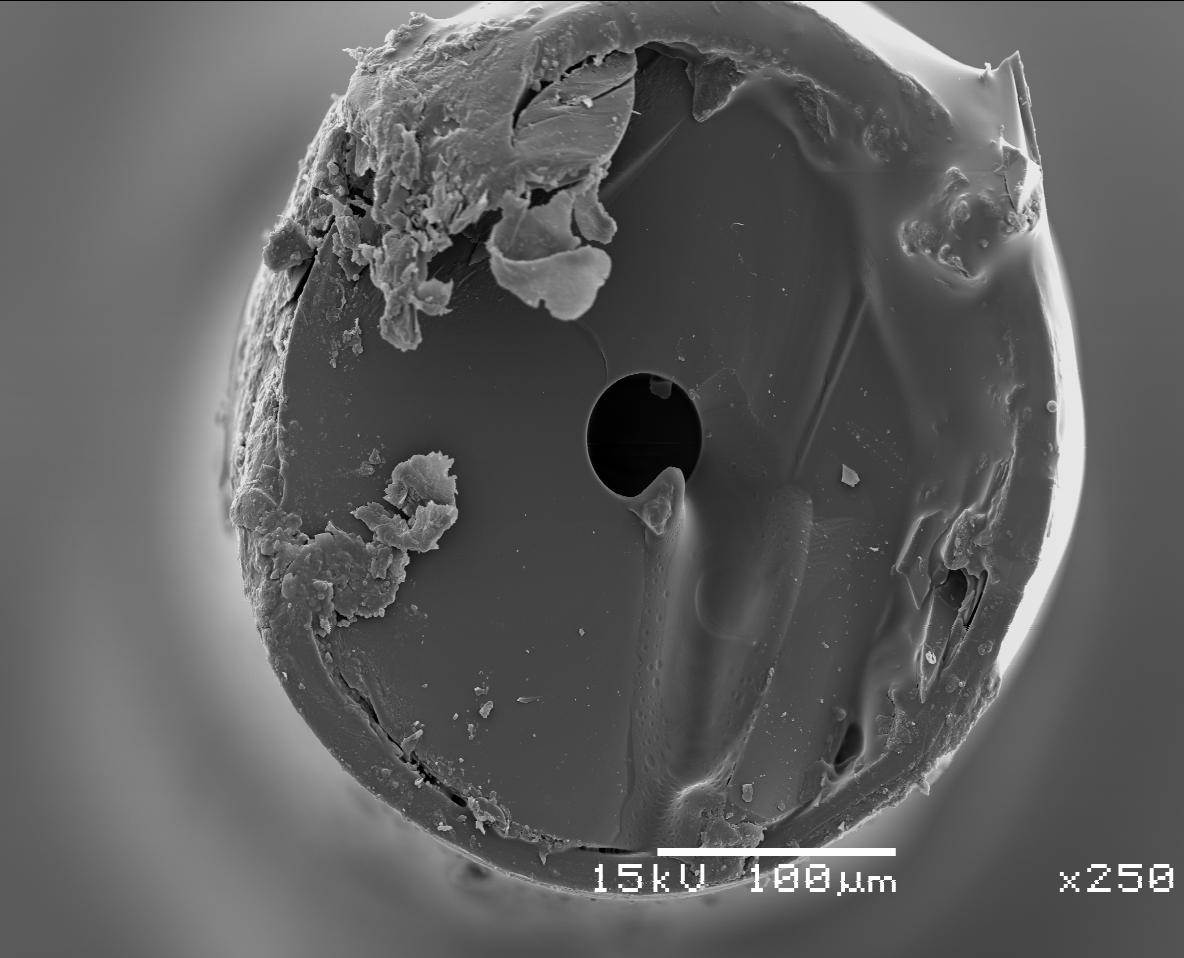
\includegraphics[width=0.8\textwidth,natwidth=4.17in,natheight=3.32in]{./Figures/A_001.pdf}
	\rule{35em}{0.5pt}
	\caption["SEM image of a capillary end."]{"A SEM image of a capillary end."}
	\label{fig:A001}
\end{figure}

A close-up image of the 

\begin{figure}[htbp]
	\centering
	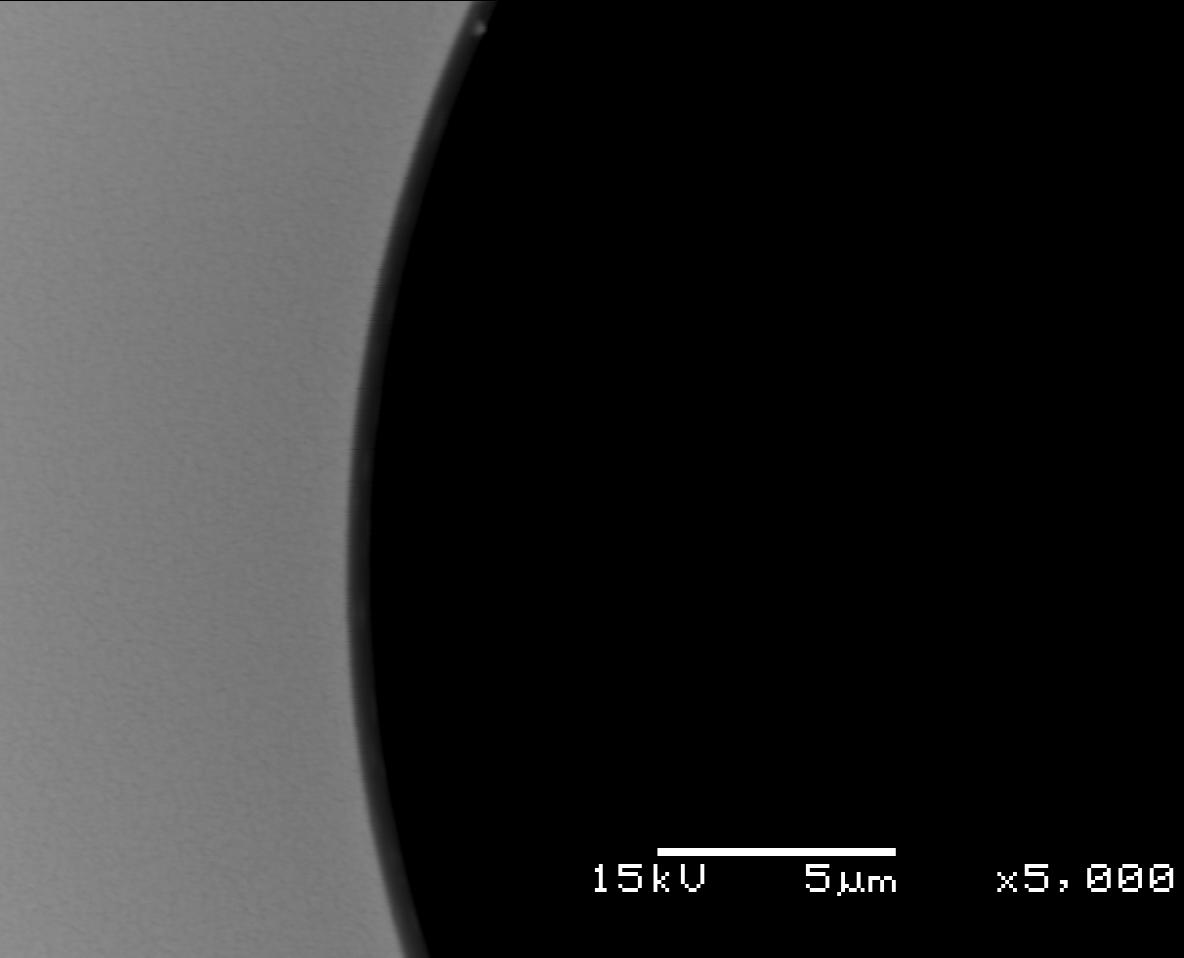
\includegraphics[width=0.8\textwidth,natwidth=4.17in,natheight=3.32in]{./Figures/A_003.pdf}
	\rule{35em}{0.5pt}
	\caption["Capillary wall"]{"A SEM image displaying the smoothness of a capillary wall."}
	\label{fig:TheFigureLabel}
\end{figure}


Since the orifices in these pictures are between 10 and 20 micron in diameter, we concluded that it was not material from the column that plugged the orifice. 

We observed one plugged restrictor with visible black material in the orifice that seemed to have been plugged by piece of stainless steel shaving. The elemental analysis suggest that the angular piece visible in the hole consisted of iron, chromium and nickel.

\begin{figure}[htbp]
	\centering
	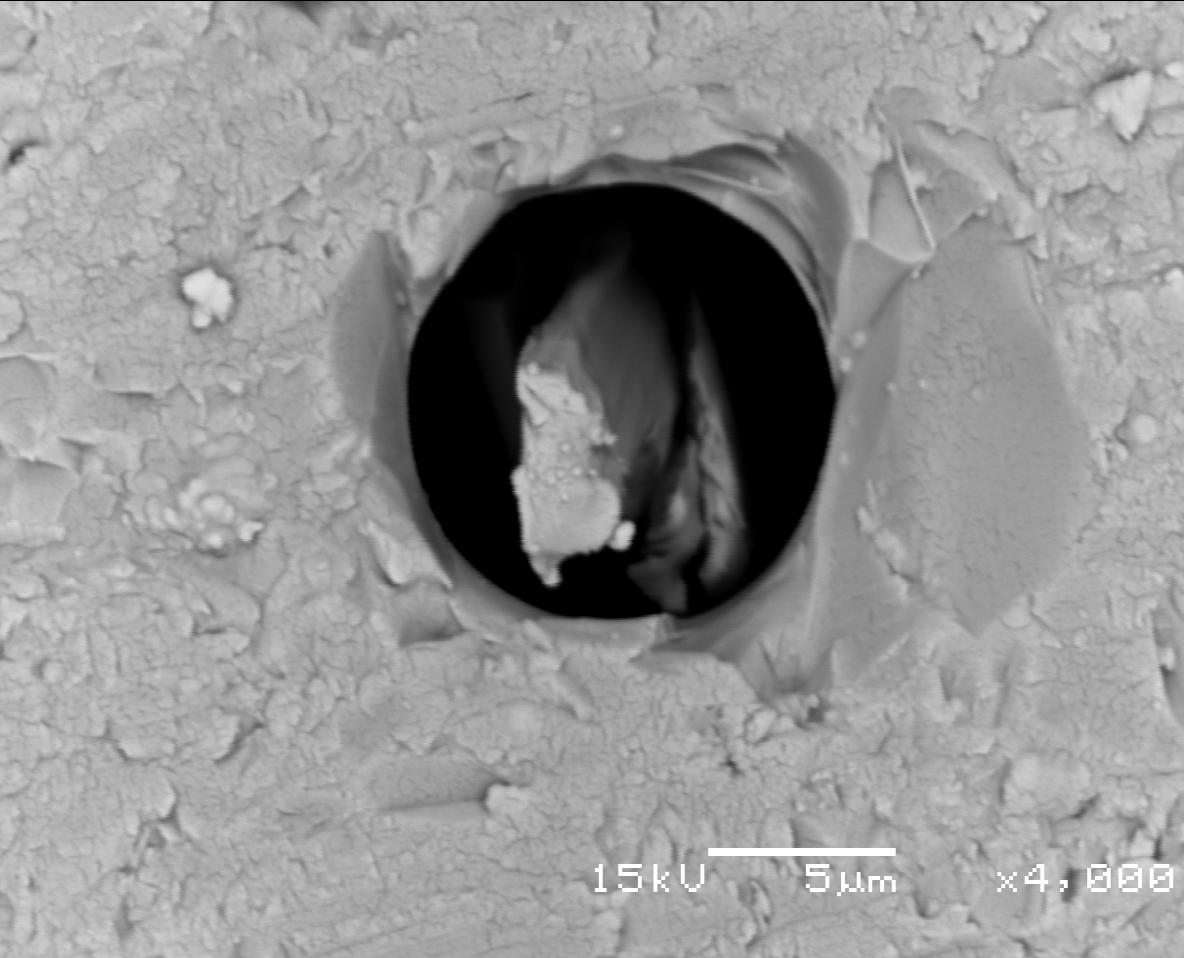
\includegraphics[width=0.8\textwidth,natwidth=4.17in,natheight=3.32in]{./Figures/H_004.pdf}
	\rule{35em}{0.5pt}
	\caption["A shaving-plugged orifice"]{"A SEM image of an orifice plugged by a shaving of stainless steel. "}
	\label{fig:H004}
\end{figure}


The plugging by colourless material, combined with the fact that plugging only appeared when the pressure in the restrictor cycled, we developed a hypothesis that the plugging was caused by material dissolved in the system which preciptated during the pressure cycle in the restrictor capillary.

This seems to be confirmed by the image of one restrictor covered by a smooth material, completely blocking the end face of the capillary.

\begin{figure}[htbp]
	\centering
	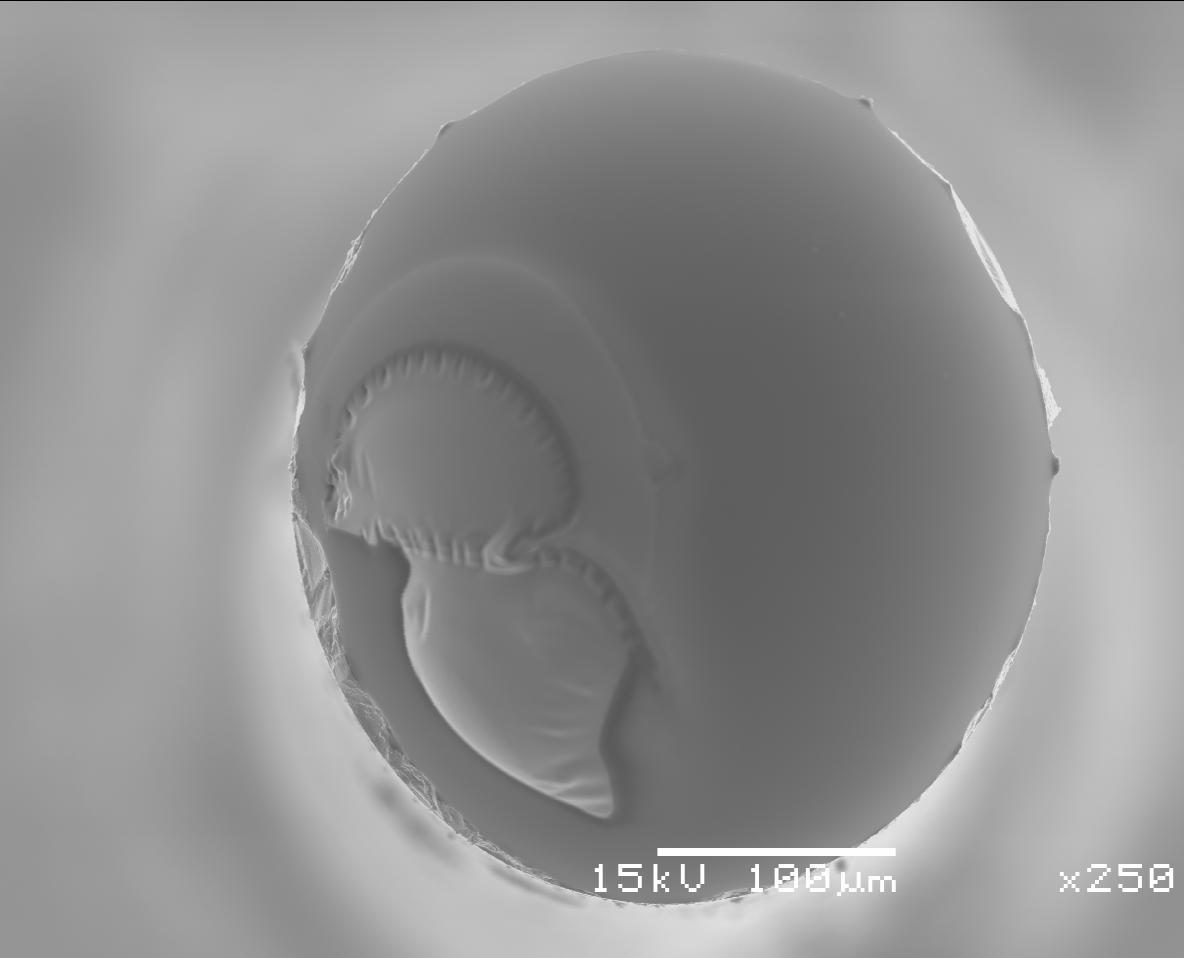
\includegraphics[width=0.8\textwidth,natwidth=4.17in,natheight=3.32in]{./Figures/F_001.pdf}
	\rule{35em}{0.5pt}
	\caption["A restrictor covered by a soft material"]{"A SEM image of an orifice completely plugged and the capillary end coated with a soft, smooth material."}
	\label{fig:F001}
\end{figure}

In addition, the inside of a capillary blocked with no visible material shows a deposit on the inside of the wall. 

\begin{figure}[htbp]
	\centering
	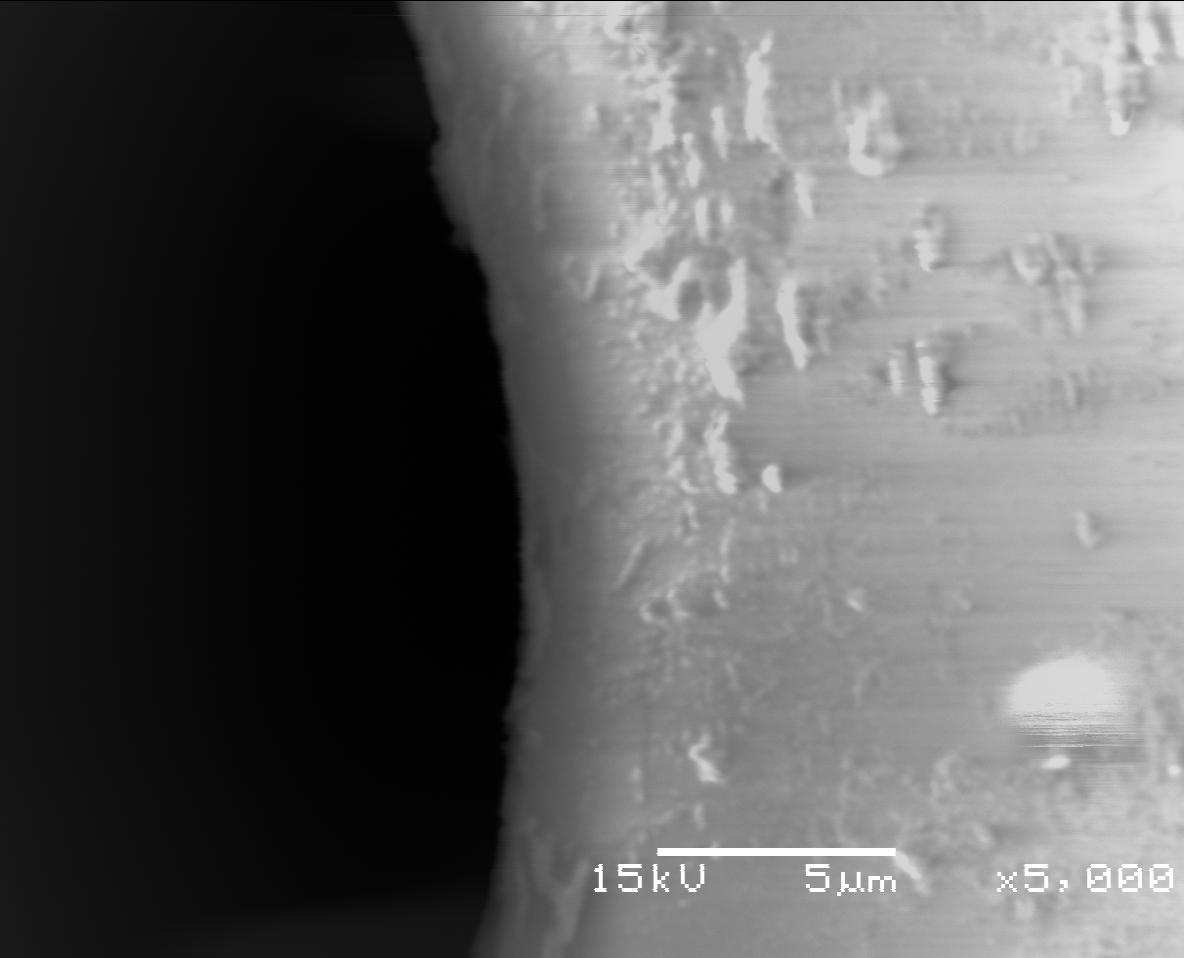
\includegraphics[width=0.8\textwidth,natwidth=4.17in,natheight=3.32in]{./Figures/D_004.pdf}
	\rule{35em}{0.5pt}
	\caption["A coating on the inside of a capillary"]{"A SEM image showing a layer precipitated on the inside wall a capillary."}
	\label{fig:D004}
\end{figure}

The smallness of the orifice contributes to the plugging problem. With a diameter of 50 $\mu$m, a solid sphere that fits in this capillary will have a volume of .065nL, or 65pL. This means that nanogram quantities of materail can easily block the restrictor. 

On re-examining our assumptions about the evaporation process, we saw the the evaporation process is not as strenuous as we thought, and the linear restrictor would probably be adequate. 

We therefore switched our restrictor choice to the linear restrictor. 1

\section{Detectors}

UV: CO2 transparency 

\section{Software} % Or should this be a separat Chapter?


The hardware described above were of course controlled by software. 

The controlling software was based on the graphical programming platform LabVIEW, version 7.11, supplied by National Instruments. This interfaced easily with the National Instruments PIC 512 E multi-IO card. 

\subsection{Instrument Control}
A number of individual PID controllers were used. The tuning of the PID controllers were done according to \cite{Peacock}.

Each controller uses an individual WHILE loop in LabVIEW. I discovered that apparently every WHILE loop runs in it's own thread, independently of the other loops in the VI, as long as there are no wires connecting two loops. In that case the loop will naturally pause until it gets data from all the wires, meaning that the running of the slower loop will determine the rate of execution of the other loop. 

The ``main loop'' in the program is the one that determines the state of the instrument.

To make sense of all the different settings in the instrument, the instrument had different `states'. The SFC had different states, and one of these states triggered and contained the states of the GC. 

The SFC had the following states:
\begin{description}
	\item[0. Idle] Pump off. Stop valve shut.
	\item[1. Equilibrate] Pump running. Stop valve open.
	\item[2. Loading] Sample valve on `Load'. GC at purge temperature. Stop valve shut.
	\item[3. Dead volume] Sample valve switches to `Inject'. Pump running. Stop valve open. 
	\item[4. Pre GC Time] Wait for dead volume time to pass.
	\item[5. Cryo] Cryo valve opens.
	\item[6. Cooling] GC column cools.
	\item[7. Collecting] Stop valve opens. 
	\item[8. Wait for GC\_sampled] Wait for collecting period.
	\item[9. Inlet flush] Stop valve shuts. Sample enters GC column. Inlet pressure rises.
	\item[10. Wait for sample to enter column]
	\item[11. Inlet vent] Inlet vent valve opens. Inlet pressure returns to normal.
	\item[12. Wait for inlet venting] Inlet vents and inlet is flushed with hydrogen.
	\item[13. GC Run] The inlet valve shuts. A GC run is started.
	\item[14. Wait for GC to finish]
	\item[15. End of GC run]
	\item[16. Emergency Stop or Initialise]
\end{description}

At the end of the GC run the state returns to `Cryo' (5), except if the set duration of the SFC run has been exceeded, in which case it switches to `Idle' (0).

The GC had the following states

\begin{description}
	\item[0. Idle] Nothing happens. GC temperature is set by an Idle Temperature control.
	\item[1. Start GC run] Toggles a flag that show that the temperature ramp is running.
	\item[2. Wait for equilibrium] Wait for the start temperature to be reached.
	\item[3. Start gradient] Set the ramp start time.
	\item[4. Run Gradient] Set temperature to current ramp temperature. Write data.
	\item[5. End Run] Write time at end of data strip. Return to `Idle' state. `
\end{description}



The coaxial heater had it's own loop to control the heating and cooling. The temperature setpoint was set by the GC ramp, via the GC `Run gradient' state.  

Each of the inlet leg and outlet leg heaters had it's own PID loop. The output of the PID loop was a percentage duty cycle used in the pulse-width modulation (PWM) of the power to the heater, implemented by switching the power to the heater on and off. This PWM had a very long period (5 seconds) , so it was adequate to implement it in software --- in industry they are more commonly implemented using hardware counter/timers. The power to the inlet and outlet leg heaters were switched on and off using solid state relays. These were easily controlled by the digital output controls of the 

The pumps had their own loop. It didn't have a PID controller. The pulses to the pump were merely switched off when the pressure exceeded the setpoint by a set amount, and switched on when it fell below the setpoint. 

\subsection{Data collection and analysis.}

Data was collected in a file using the following format:

\begin{tabular}{|l|l|l|l|}
\hline
No & Data Type & Value & Units \\
\hline
1 & Integer8 & ID & None \\
2 & Real64 & Time & s \\
3 & Real64 & TAmbient & K  \\
4 & Real64 & Ttc & K \\
5 & Real64 & Vb & V \\
6 & Real64 & dV & V \\
7 & Real64 & P1 & Pa \\
8 & Real64 & P2 & Pa \\
9 & Real64 & TInlet & K \\
10 & Real64 & TOutlet & K \\
11 & Real64 & Detector & V \\
12 & Real64 & TColumn & K \\
13 & Real64 & P1 Setpoint & Pa \\
14 & Real64 & P2 Setpoint & Pa \\
15 & Real64 & TInlet Setpoint & K \\
16 & Real64 & TOutlet Setpoint & K \\
17 & Real64 & TColumn Setpoint & K \\
\hline

\end{tabular}

The values TAmbient to Detector are digitized measurements. TColumn is calculated from Vb and dV by the calibration formula. P1 setpoint to TColumn Setpoint are the setpoints from the control system. Including the setpoints makes the data files larger, but it gives invaluable information on the quality of the controlled quantities, and can greatly assist {\it post hoc} debugging.

In this table TAmbient is the temperature measured by the thermistor used for cold junction compensation. Ttc is the temperature of a free thermocouple used for measuring temperatures in various places. Vb is the voltage of the current-measuring circuit, and dV is the voltage of the voltage-measuring circuit of the coaxial heater. P1 is the pressure measured by the first piston pump, and P2 is the pressure measured by the modifier pump. TInlet and Toutlet are the temperatures of the inlet and outlet leg heaters respectively. 

The �Time� meaning depends on the �ID�. 

\begin{tabular}{|l|l|l|}

\hline
ID & Time Value & Meaning \\
\hline
0 & 0 & File Created \\
1 & SFC\_Run\_Time � Interval & Time of start of GC run \\
2 & Current time � GC\_Time0 & Data point of GC run \\
3 & SFC\_Run\_Time/60000 & End of GC run? \\
4 & SFC\_Run\_Time & End of SFC run \\
\hline

\end{tabular}

Naturally most of the data points would have ID = 2, and the rest are just time stamps to identify the times of the start of the end of the runs. 

This data structure is simple but not particularly portable, as is evident by the following note given in the LabVIEW documenation:
\begin{quote}
Note: LabVIEW uses the big-endian format when handling and storing multi-byte data, even on the Windows (x86) platform. Little Endian was the choice for computers based on the Intel x86 processors, while Motorola processors (including the Macintosh computer, for which LabVIEW was first developed) used big-endian. Be aware that C and other Windows applications typically expect numeric data to be in little-endian form.
\end{quote}

Source: http://digital.ni.com/public.nsf/allkb/8224F2391418FDF6862568F00051D091

Therefore the data was converted into the ANDI (netCDF) format. This format can be read by the ChromaTOF software by LECO, giving us access to a well-developed tool for 2D data analysis.

The conversion was done it a two-step process, to avoid having to develop custom software for a poorly-defined data file with a structure that's still in development. Using Mathematica, the data was written from LabVIEW binary to a NCL text file, which was then converted to netCDF using the utility ncGen. This generated a properly-formatted netCDf file. 

 % Instrumentation: Gardient elution SFC

% Chapter 5

\chapter{Instrumentation Performance} % Write in your own chapter title
\label{Chapter5}
\lhead{Chapter 5. \emph{Performance}} % Write in your own chapter title to set the page header

\section{SFC}

\subsection{Restrictor blockage}

Figure~\ref{fig:RestrictorEnd} is a SEM image of the end of the restrictor used to depressurize the supercritical carbon dioxide. 

\begin{figure}[htbp]
	\centering
	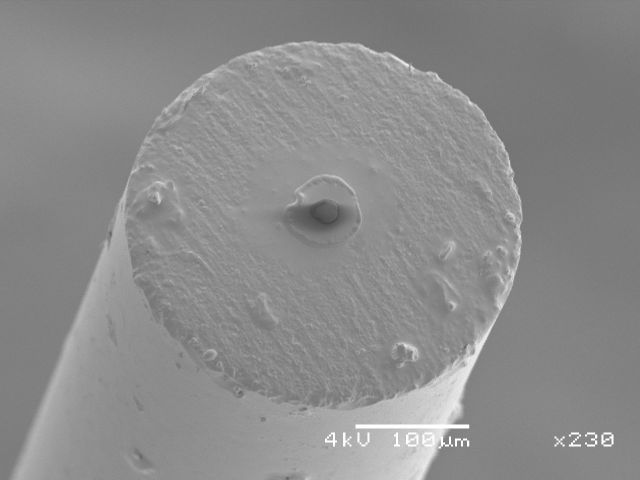
\includegraphics[width=0.8\textwidth,natwidth=4.17in,natheight=3.32in]{./Figures/RestrictorEnd.jpg}
	\rule{35em}{0.5pt}
	\caption[A SEM image of a restrictor orifice]{A SEM image of a restrictor orifice. The grinding marks of the 2000 grit grinding medium can be clearly seen on the end of the capillary. The left-to-right dark `smudge' around the orifice is cause by some charging of the hole in the electorn microscope, because the gold sputtering process does not coat the inside of holes very easily.}
	\label{fig:RestrictorEnd}
\end{figure}

From time to time this restrictor got plugged. Initially it was though that this plugging was caused by particles from the valve system and the columns, and the plugging . The size of the hole was not known, because the end of the restrictor was ground down until the hole was the right size for the desired flow. What was known was that the hole was too small to be visible to the naked eye or under a low-power stereo microscope. A higher-powered stereo microscope at the Unit for Microscopy and Microanalysis at the University of Pretoria showed that the hole is about 10 to 20 micron in diameter, which answered one question: since the 0.5$\mu$m filter should remove all the smaller particles, a 20 $\mu$m orifice will easily pass any particles let through by the filter. Even the 3 $\mu$m column packing particles will not plug this hole. Therefore it seems very unlikely that single particles cause the plugging.

The possibility exists that an excess of small particles may clot and form a plug. 

Taking the SEM image confirmed the size of the hole, but revealed something else. This particular restrictor had plugged, but had been ground again to recover flow. Around the hole there is visible an `island' of different texture. A SEM image in backscatter mode (Figure~\ref{fig:RestrictorHole}) shows that the chemistry of this `island' is different from the chemistry of the surrounding silica. The morphology also suggests that it is a much softer material, it not exhibiting grinding marks and appearing to have flowed.

\begin{figure}[htbp]
	\centering
	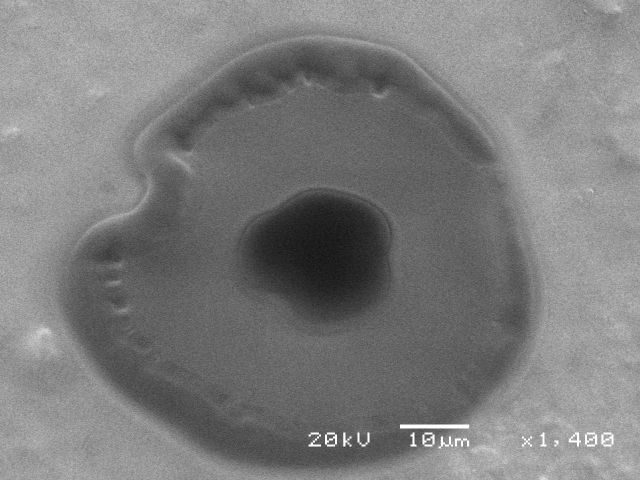
\includegraphics[width=0.8\textwidth,natwidth=4.17in,natheight=3.32in]{./Figures/RestrictorHole.jpg}
	\rule{35em}{0.5pt}
	\caption[Restrictor Ofrifice]{The end of restrictor, showing the size of the orifice.}
	\label{fig:RestrictorHole}
\end{figure}

What is clear is that there is no evidence of particulate matter plugging the orifice.

There is a possibility that this softer material is the actual blocking matter. There are some proposed origins for this material.
\begin{itemize}
	\item It might be polymeric material formed in the sample that got transported through the system and precipitated in the restrictor. (We have found polymeric material in essential oils.)
	\item It might be sample material that separated in the SFC column, but precipitated during the SFC cycling on and off, and failed to re-dissolve during subsequent cycles because conditions different from the injection and separation parts of the SFC made dissolution kinetically unfavourable.
	\item It might be sample material that precipitated during the pressure cycles of the SFC going into stopped-flow, and then polymerised or carbonised in the hot inlet.
	\item It might be that the capillary is not manufactured of uniform material but contains a softer core around the lumen of the capillary.
\end{itemize}

\section{Fast GC}

\section{Heating and cooling rates}

In previous work using SFC�GC, the metal column was cooled by using the cryogenic cooling function of the Varian 3300 oven. This function works by injection liquid carbon dioxide into the oven, behind the air circulating fan. This ensures a cooling of the whole oven. But this function of the Varian was intended for the cooling of the oven once for every normal GC run, which would mean cooling at most every 10 minutes or so. Using the fast GC column to trap small fractions of SFC eluent means the very frequent cooling of the whole oven. Although the oven is not deliberately heated, heat from the heated inlet and detector would still leak into the oven.

These workers reported [Makgwane2006] that the system used a lot of carbon dioxide for cooling.

When we started using the coaxial capillary heater, we welded wires to the stainless steel heater capillary. To prevent creating cold spots on the column, we added heater blocks to the junctions, close to the inlet and detector, to ensure an evenly heated area where the conductor joins the coaxial heater. Though it was thermally isolated, more heat still leaked into the oven. 

In our experience, the total cooling required for this system was about half a bottle (approximately 16 kg) of technical grade carbon dioxide per 2D chromatographic run. 

This is an unacceptably high consumption of carbon dioxide, both in terms of cost and of unnecessary carbon emission. That costs about ZAR 3.56 just in carbon costs per run. 

% On the 1st of July 2012 the Australian Federal government introduced a carbon price, a price of $23AUD per tonne of emitted CO2-e on selected fossil fuels consumed by major industrial emitters only.
% That's ZAR 216 per tonne. 21.6 per kilogram. 

So it was decided to take the step to cool the column only, using the concept of the capillary coaxial heater, and then blowing the liquid carbon dioxide into the void between the heater and the column. 

The flow needed for this about one tenth of the flow used by the Varian's cryogenic cooling, and the duration of the flow is much less, resulting in a lesser use of carbon dioxide for cooling. 

%Figure showing flow compared between Varian and coaxial cooling. 
\begin{figure}[htbp]
	\centering
%	\includegraphics[width=0.8\textwidth,natwidth=4.17in,natheight=3.32in]{./Figures/filename.pdf}
	\rule{35em}{0.5pt}
	\caption["short"]{"long"}
	\label{fig:TheFigureLabel}
\end{figure}

% Add calculation to show 

The saving in carbon dioxide is significant, but the effort saved in not needing to worry about the coolant running out saves much more effort and energy. A sample run can easily be ruined by the coolant running out unexpectedly. And as we know, there is no way of determining the contents level of an industrial steel cylinder of liquefied gas. 

\section{Repeatability}

In the work by Venter \cite{Venter2004}\cite{Venter2006} it became apparent that the temperature programme was not too reliable. This was pointed out in a graph that compared the temperature reported by the controlling thermocouple with the temperature reported by a monitoring thermocouple positioned on another part of the metal column. Although the temperature of the controlling thermocouple followed the setpoint of the temperature ramp faithfully, the monitoring thermocouple reported quite a different temperature. The 2D chromatogram of course showed this discrepancy, with the contouring software interpreting the jaggedness of the resulting peaks as separate peaks. 

 % Instrumentation performance

% Chapter 6

\chapter{Analysis of Biodiesel} % Write in your own chapter title
\label{Chapter6}
\lhead{Chapter 6. \emph{Biodiesel analysis}} % Write in your own chapter title to set the page header


\section{Introduction to Biodiesel}

\section{Fatty acid profiles.}

The driving force of comprehensive 2D chromatography is orthogonality, the principle that two different separation mechanisms used successively will give greater separation power. The more different the separation mechanisms are, the higher the orthogonality. 

In \GCxGC there is always a tendency for low orthognality. This is because the basic separation mechanism of capillary chromatography is partion chromatography, and compounds with higher molecular weight tend to have longer retention times.

When using adsorption chromatography, however, the intermolecular forces are much higher, and molecular weight plays a lesser role in retention time.

A good example of this is Roger Smith's work that has proven that FAMEs separated by SFC, using pure carbion dioxide as a mobile phase and silica as a stationary phase, elute in order of number of double bonds, independent of the chain length.  % Analysis of biodiesel

% Chapter 7

\chapter{Conclusion} % Write in your own chapter title
\label{Chapter7}
\lhead{Chapter 7. \emph{Conclusion}} % Write in your own chapter title to set the page header


\section{Introduction to Biodiesel}
 % Conclusion

%% ----------------------------------------------------------------
% Now begin the Appendices, including them as separate files

\addtocontents{toc}{\vspace{2em}} % Add a gap in the Contents, for aesthetics

\appendix % Cue to tell LaTeX that the following 'chapters' are Appendices

% Appendix A

\chapter{Appendix Title Here}
\label{AppendixA}
\lhead{Appendix A. \emph{Appendix Title Here}}

Write your Appendix content here.	% Appendix Title

%\input{./Appendices/AppendixB} % Appendix Title

%\input{./Appendices/AppendixC} % Appendix Title

\addtocontents{toc}{\vspace{2em}}  % Add a gap in the Contents, for aesthetics
\backmatter

%% ----------------------------------------------------------------
\label{Bibliography}
\lhead{\emph{Bibliography}}  % Change the left side page header to "Bibliography"
\bibliographystyle{unsrtnat}  % Use the "unsrtnat" BibTeX style for formatting the Bibliography
\bibliography{SFCGC}  % The references (bibliography) information are stored in the file named "Bibliography.bib"
\end{document}  % The Ends
%% ----------------------------------------------------------------